% !Mode:: "Tex:UTF-8"



\documentclass[10pt,a4paper]{article}\usepackage[]{graphicx}\usepackage[]{color}
%% maxwidth is the original width if it is less than linewidth
%% otherwise use linewidth (to make sure the graphics do not exceed the margin)
\makeatletter
\def\maxwidth{ %
  \ifdim\Gin@nat@width>\linewidth
    \linewidth
  \else
    \Gin@nat@width
  \fi
}
\makeatother

\definecolor{fgcolor}{rgb}{0.345, 0.345, 0.345}
\newcommand{\hlnum}[1]{\textcolor[rgb]{0.686,0.059,0.569}{#1}}%
\newcommand{\hlstr}[1]{\textcolor[rgb]{0.192,0.494,0.8}{#1}}%
\newcommand{\hlcom}[1]{\textcolor[rgb]{0.678,0.584,0.686}{\textit{#1}}}%
\newcommand{\hlopt}[1]{\textcolor[rgb]{0,0,0}{#1}}%
\newcommand{\hlstd}[1]{\textcolor[rgb]{0.345,0.345,0.345}{#1}}%
\newcommand{\hlkwa}[1]{\textcolor[rgb]{0.161,0.373,0.58}{\textbf{#1}}}%
\newcommand{\hlkwb}[1]{\textcolor[rgb]{0.69,0.353,0.396}{#1}}%
\newcommand{\hlkwc}[1]{\textcolor[rgb]{0.333,0.667,0.333}{#1}}%
\newcommand{\hlkwd}[1]{\textcolor[rgb]{0.737,0.353,0.396}{\textbf{#1}}}%
\let\hlipl\hlkwb

\usepackage{framed}
\makeatletter
\newenvironment{kframe}{%
 \def\at@end@of@kframe{}%
 \ifinner\ifhmode%
  \def\at@end@of@kframe{\end{minipage}}%
  \begin{minipage}{\columnwidth}%
 \fi\fi%
 \def\FrameCommand##1{\hskip\@totalleftmargin \hskip-\fboxsep
 \colorbox{shadecolor}{##1}\hskip-\fboxsep
     % There is no \\@totalrightmargin, so:
     \hskip-\linewidth \hskip-\@totalleftmargin \hskip\columnwidth}%
 \MakeFramed {\advance\hsize-\width
   \@totalleftmargin\z@ \linewidth\hsize
   \@setminipage}}%
 {\par\unskip\endMakeFramed%
 \at@end@of@kframe}
\makeatother

\definecolor{shadecolor}{rgb}{.97, .97, .97}
\definecolor{messagecolor}{rgb}{0, 0, 0}
\definecolor{warningcolor}{rgb}{1, 0, 1}
\definecolor{errorcolor}{rgb}{1, 0, 0}
\newenvironment{knitrout}{}{} % an empty environment to be redefined in TeX

\usepackage{alltt}
\usepackage{etoolbox}
\newtoggle{color}
%\togglefalse{color}
\toggletrue{color}

\usepackage{makeidx}
\newcommand{\idioma}{spanish}
\newcommand{\opcionesIdioma}{,es-nodecimaldot,es-tabla}
% !Mode:: "Tex:UTF-8"
%%%%%%%%%%%%%%%%%%%%%Carga de Packages
%%poner \newcommand{\idioma}{spanish} o \newcommand{\idioma}{english} en el documento
\usepackage{pdfsync}
\usepackage{srcltx}
\usepackage[\idioma\opcionesIdioma]{babel}
\usepackage[utf8x]{inputenc}
\usepackage[T1]{fontenc}
\usepackage{graphicx}
\graphicspath{{/users/fernando/figuras/}{./}{./figuras/}{/fernando/figuras/}{/fernando/figuras/jpg/}}
\usepackage{multicol}
\usepackage{epsfig}
%\usepackage{oberdiek}
\usepackage{listingsutf8}
\lstset{inputencoding=utf8/latin1}
%\lstset{extendedchars=true}
\lstset{ %
  language=R,                     % the language of the code
  basicstyle=\ttfamily\small,       % the size of the fonts that are used for the code
  numbers=left,                   % where to put the line-numbers
  numberstyle=\tiny\color{gray},  % the style that is used for the line-numbers
  stepnumber=1,                   % the step between two line-numbers. If it's 1, each line
                                  % will be numbered
  numbersep=5pt,                  % how far the line-numbers are from the code
  backgroundcolor=\color{white},  % choose the background color. You must add \usepackage{color}
  showspaces=false,               % show spaces adding particular underscores
  showstringspaces=false,         % underline spaces within strings
  showtabs=false,                 % show tabs within strings adding particular underscores
  frame=single,                   % adds a frame around the code
  rulecolor=\color{black},        % if not set, the frame-color may be changed on line-breaks within not-black text (e.g. commens (green here))
  tabsize=2,                      % sets default tabsize to 2 spaces
  %captionpos=,                   % sets the caption-position to bottom
  breaklines=true,                % sets automatic line breaking
  breakatwhitespace=false,        % sets if automatic breaks should only happen at whitespace
  %title=\lstname,                 % show the filename of files included with \lstinputlisting;
                                  % also try caption instead of title
  keywordstyle=\color{black},      % keyword style
  commentstyle=\color{Brown},   % comment style
  stringstyle=\color{black},      % string literal style
  escapeinside={\%*}{*)},         % if you want to add a comment within your code
  morekeywords={*,...},            % if you want to add more keywords to the set
  lineskip={-2.5pt} % single line spacing
}
%\usepackage{algorithm}
\usepackage{amsmath}
\usepackage{amsfonts}
\usepackage{amssymb}
\usepackage{amsthm}
\usepackage{fancybox}
\usepackage{fancyvrb}
\usepackage{rotating}
\usepackage{keystroke}
\usepackage{array}
\input{xy}
\xyoption{all}
%\usepackage[dvipsnames,usenames]{color}
\usepackage[usenames,dvipsnames,svgnames,table]{xcolor}
\usepackage{colortbl}
\usepackage{comment}
\excludecomment{spanish}
\excludecomment{english}
\includecomment{\idioma}

%\usepackage{noweb}
%\usepackage{clrscode}
\usepackage{eurosym}
\usepackage{wasysym}
\usepackage{multirow}
%\usepackage{margins}
\usepackage{lscape}
\usepackage{longtable}
\usepackage[normalem]{ulem}
\usepackage{xr-hyper}

%%NUEVO
\newcolumntype{C}{{\centering\arraybackslash}m{20mm}}
\newcommand{\centercell}[1]{\multicolumn{1}{c}{#1}}
\newcommand{\colHead}[1]{\centercell{\bfseries#1}}

\excludecomment{ocultar}


% Matriz (par‚ntesis)
\def\matr#1#2{\left(\begin{array}{#1}#2\end{array}\right)}
% Determinante (barras)
\def\deter#1#2{\left|\begin{array}{#1}#2\end{array}\right|}
% Sistema de ecuaciones. (llave a la izda.)
\def\seq#1#2{\left\{\begin{array}{#1}#2\end{array}\right.}
% Ecuaci\'on de varias lineas (sin llave a la izda.)
\def\evl#1#2{\begin{array}{#1}#2\end{array}}

%%%%%%%%%%%%%%%%%%%%%%%%%%%%%%%%%%%%%%%%%%%%%%
%%%%%%%%%%%%%%%%%%%%%%%%%%%%%%%%%%%%%%%%%%%%%%
%%%%%%%%%%%%%%%%% M\'{a}rgenes %%%%%%%%%%%%%%%%
%
%
%\parindent=0mm
%
%\textwidth=160mm
%\textheight=220mm
%\hoffset=-20mm
%\voffset=-15mm
%\parskip=0mm
\marginparsep=3mm
\marginparwidth=25mm
%
%%%%%%%%%%%%%%%%%%%%%%%%%%%% Contadores para listas de problemas
%\newcommand{\adc}{\addtocounter{enumi}{1}}
\newcommand{\adc}{\stepcounter{enumi}}
\newcommand{\adci}{\stepcounter{enumii}}
\newcommand{\xadc}{\addtocounter{xcounter}{1}}
\newcommand{\be}{\begin{enumerate}}
\newcommand{\ee}{\end{enumerate}}
\newcommand{\bi}{\begin{itemize}}
\newcommand{\ei}{\end{itemize}}
\newcounter{xcounter}


\newcommand{\nin}{{\noindent}}

%\newcounter{prob}{}
%\def\pr{\addtocounter{prob}{1}(\theprob)\ }
%\def\pr2{\addtocounter{prob}{2}(\theprob)\ }

%%%%%%%%%%%%%%%%%%%%%%%%%%%Fin de demostraciones, ejemplos, etc.
\newcommand{\fin}{$\square$}
%%%%%%%%%%%%%%%%%%%%%%%%%%Notaci\'{o}n matem\'{a}ticas generales
%\newcommand{\suc}[1]{\{#1_n\}}
%\newcommand{\sucn}[1]{\{#1_n\}_{n\in\mathbb{N}}}
%\newcommand{\ser}[1]{\sum #1_n}
%\newcommand{\sern}[1]{\sum_{n\geq 1} #1_n}
%\newcommand{\limn}{\lim_{n\rightarrow\infty}}
%\newcommand{\limnd}{\displaystyle\lim_{n\rightarrow\infty}}
%\newcommand{\mf}[1]{\mathbf{#1}}
%\newcommand{\mb}[1]{\mathbb{#1}}
%\newcommand{\D}[1]{\Dv_{\mf{#1}}}
%\newcommand{\bsigma}{\pmb{\sigma}}
%\newcommand{\bPhi}{\pmb{\Phi}}
%\newcommand{\vol}{\operatorname{vol}}
%\newcommand{\ldbr}{[\hspace{-1.5pt}[}
%\newcommand{\rdbr}{]\hspace{-1.5pt}]}
%\newcommand{\fpws}[2]{{#1}\ldbr{#2}\rdbr}
%\newcommand{\leftPui}{<\hspace{-3pt}<}
%\newcommand{\rightPui}{\hspace{-3pt}}
%\newcommand{\Pui}[2]{{#1}\hspace{-6pt}\leftPui{#2}\rightPui}
%\newcommand{\pdd}[2]{\dfrac{\partial{#1}}{\partial{#2}}}
%%%%%%%%%%Conjuntos de n\'{u}meros
\newcommand{\N}{\mathbb{N}} %conjunto de n\'{u}meros naturales
\newcommand{\Z}{\mathbb{Z}} %conjunto de n\'{u}meros enteros
\newcommand{\R}{\mathbb{R}} %conjunto de n\'{u}meros reales
\newcommand{\C}{\mathbb{C}} %conjunto de n\'{u}meros complejos
\newcommand{\Q}{\mathbb{Q}} %conjunto de n\'{u}meros racionales
\newcommand{\EP}{\mathbb{P}} %espacios proyectivos
\newcommand{\K}{\mathbb{K}} %cuerpo gen\'{e}rico
\newcommand{\A}{\mathbb{A}} %espacios afines

%%%%%%%%%%Estadistica
\newcommand{\MEAN}{\mathrm{E}}
\newcommand{\Var}{\mathrm{Var}}
\newcommand{\Cov}{\mathrm{Cov}}


%%%%%%%%%%Funciones
\def\arcsen{\operatorname{arcsen}}
\def\arctg{\operatorname{arctg}}
\def\argCosh{\operatorname{argCosh}}
\def\argSenh{\operatorname{argSenh}}
\def\argTgh{\operatorname{argTgh}}
\def\cosec{\operatorname{cosec}}
\def\Cosh{\operatorname{Cosh}}
\def\cotg{\operatorname{cotg}}
\def\Dv{\operatorname{D}}
\def\discrim{\operatorname{discrim}}
\def\dive{\operatorname{div}}
\def\dom{\operatorname{dom}}
\def\Ext{\operatorname{Ext}}
\def\Fr{\operatorname{Fr}}
\def\dder#1#2{\dfrac{d #1}{d #2} } %derivada en estilo display
\def\gr{\operatorname{gr}}
\def\grad{\operatorname{grad}}
\def\Imag{\operatorname{Im}}
\def\mcm{\operatorname{mcm}}
\def\rang{\operatorname{rang}}
\def\rot{\operatorname{rot}}
\def\sen{\operatorname{sen}}
\def\Senh{\operatorname{Senh}}
\def\sgn{\operatorname{sgn}}
\def\sig{\operatorname{sig}}
\def\tg{\operatorname{tg}}
\def\Tgh{\operatorname{Tgh}}
\def\E{\operatorname{E}}
\def\VAR{\operatorname{VAR}}
\newcommand{\margWeb}[2]{\noindent{#2}\marginpar[\hspace{-18mm}\link{#1}{WEB}]{\hspace*{-18mm}\link{#1}{WEB}}}

%%%%%%%%%%%%%%%%%%%%%%\'{A}lgebra conmutativa.
\def\multideg{\operatorname{multideg}} %multidegree of a polynomial
\def\LT{\operatorname{lt}} %leading term of a polynomial
\def\LC{\operatorname{lc}} %leading coefficient of a polynomial
\def\LM{\operatorname{lm}} %leading monomial of a polynomial
\def\Mexp{\mathbb{Z}^n_{\geq 0}} %set of multiexponents of monomials
\def\set#1{\left\{{#1}\right\}}
\newcommand{\vlist}[2]{\mbox{${#1}_{1},\ldots,{#1}_{#2}$}}
\def\deg{\operatorname{deg}} %grado de un polinomio
\def\cp{\operatorname{cp}} %coeficiente principal de un polinomio
\def\CP{\operatorname{cp}} %coeficiente principal de un polinomio
\def\set#1{\left\{{#1}\right\}} %llaves de conjunto
\newcommand{\V}{{\bf V}} %variedad de un conjunto de polinomios
\newcommand{\I}{{\bf I}} %ideal de un conjunto
\newcommand{\MCD}{\operatorname{mcd}} %m\'{a}ximo com\'{u}n divisor
\newcommand{\MCM}{\operatorname{mcm}} %m\'{\i}nimo com\'{u}n m\'{u}ltiplo
\newcommand{\LCM}{\operatorname{lcm}} %least common multiple
\newcommand{\GCD}{\operatorname{gcd}} %greatest common divisor
\newcommand{\Ker}{\operatorname{Ker}} %N\'{u}cleo
\newcommand{\IM}{\operatorname{IM}} %Imagen
\newcommand{\Rad}{\operatorname{Rad}} %radical de un ideal
\newcommand{\Jac}{\operatorname{Jac}} %radical de Jacobson de un anillo
\newcommand{\Ann}{\operatorname{Ann}} %anulador de un ideal
\newcommand{\Res}{\operatorname{Res}} %resultante de polinomios
\newcommand{\Mult}{\operatorname{mult}} %multiplicidad
\newcommand{\Gen}{\operatorname{Gen}} %g\'{e}nero
\newcommand{\Card}{\operatorname{Card}} %cardinal
\newcommand{\ord}{\operatorname{ord}} %orden
\newcommand{\prim}{\operatorname{prim}} %parte primitiva
\newcommand{\NP}{\operatorname{NP}} %NP idea
\newcommand{\cont}{\operatorname{cont}} %parte primitva
\newcommand{\pp}{\operatorname{pp}} %parte primitva
\newcommand{\PP}{\mathop{\mathrm{PP}}\nolimits}
\newcommand{\Int}{\operatorname{Int}}
\newcommand{\Ind}{\operatorname{index}}
\newcommand{\Lcoeff}{\operatorname{lc}} %leading coefficient of a polynomial
\newcommand{\Sqf}{\operatorname{Sqf}} %square free part of a polynomial

\def\pd#1#2{\frac{\partial #1}{\partial #2}} %derivada parcial
\def\mult{\text{mult}} %multiplicity
\def\Sing{\text{Sing}} %multiplicity
\def\Cl#1{\overline{#1}} %cierre topol\'{o}gico
\def\fobox#1{\begin{center}\fbox{$\displaystyle #1 $}\end{center}}

%\newcommand{\Ext}{\operatorname{Ext}}

%%%%%%%%%%%%%%%%%%%%%%%%
%% unpunto mayor que cdot, pero menor que bullet
\newcommand{\sbt}{\,\begin{picture}(-1,1)(-1,-3)\circle*{3}\end{picture}\ }

%%%%%%%%%%%%%%%%%%%%%%%%S\'{\i}mbolos rodeados de un c\'{\i}rculo
\def\circled#1{\xymatrix{*+[o][F]{#1}}}

%%%%%%%%%%%%%%%%%%%Geometr\'{\i}a
\newcommand{\CH}{{\cal CH}} %%cierre convexo

%%%%%%%%%%%%%%%%%%%%Tipos de letra especiales
%%Caligr\'{a}ficas
\newcommand{\cA}{{\cal A}}
\newcommand{\cB}{{\cal B}}
\newcommand{\cC}{{\cal C}}
\newcommand{\cD}{{\cal D}}
\newcommand{\cE}{{\cal E}}
\newcommand{\cF}{{\cal F}}
\newcommand{\cG}{{\cal G}}
\newcommand{\cH}{{\cal H}}
\newcommand{\cI}{{\cal I}}
\newcommand{\cJ}{{\cal J}}
\newcommand{\cK}{{\cal K}}
\newcommand{\cL}{{\cal L}}
\newcommand{\cM}{{\cal M}}
\newcommand{\cN}{{\cal N}}
\newcommand{\cO}{{\cal O}}
\newcommand{\cP}{{\cal P}}
\newcommand{\cQ}{{\cal Q}}
\newcommand{\cR}{{\cal R}}
\newcommand{\cS}{{\cal S}}
\newcommand{\cT}{{\cal T}}
\newcommand{\cU}{{\cal U}}
\newcommand{\cV}{{\cal V}}
\newcommand{\cW}{{\cal W}}
\newcommand{\cX}{{\cal X}}
\newcommand{\cY}{{\cal Y}}
\newcommand{\cZ}{{\cal Z}}

%%%%%%%%%%%%%%%%%%%%%%%%%%Notaci\'{o}n matem\'{a}ticas generales
\newcommand{\sucn}[1]{\{#1_n\}_{n\in\mathbb{N}}}
\newcommand{\ser}[1]{\sum #1_n}
\newcommand{\sern}[1]{\sum_{n\geq 1} #1_n}
\newcommand{\limn}{\lim_{n\rightarrow\infty}}
\newcommand{\mf}[1]{\mathbf{#1}}
\newcommand{\mb}[1]{\mathbb{#1}}
\newcommand{\D}[1]{\Dv_{\mf{#1}}}
\newcommand{\bsigma}{\pmb{\sigma}}
\newcommand{\bPhi}{\pmb{\Phi}}
\newcommand{\vol}{\operatorname{vol}}
\newcommand{\ldbr}{[\hspace{-1.5pt}[}
\newcommand{\rdbr}{]\hspace{-1.5pt}]}
\newcommand{\fpws}[2]{{#1}\ldbr{#2}\rdbr}
\newcommand{\leftPui}{<\hspace{-3pt}<}
\newcommand{\rightPui}{\hspace{-3pt}}
\newcommand{\Pui}[2]{{#1}\hspace{-6pt}\leftPui{#2}\rightPui}
\newcommand{\pdd}[2]{\dfrac{\partial{#1}}{\partial{#2}}}


%\newcounter{contEnlace}

%\newcommand{\pendiente}{\textcolor{purple}{PENDIENTE: }}
%\newcommand{\link}[2]{\textcolor{blue}{{\href{#1}{#2}}}}


\iftoggle{color}{%
  % color version
  \newcommand{\pendiente}{\textcolor{red}{PENDIENTE: }}
  \newcommand{\link}[2]{\textcolor{blue}{{\href{#1}{#2}}}}
  \newcommand{\fichero}[2]{\textattachfile{#1}{\textcolor{blue}{#2}}}
  \newcommand{\otrofichero}[2]{\textattachfile{./datos/#1}{\textcolor{blue}{#2}}}
}{%
  % b/w version
  \newcommand{\pendiente}{\textcolor{black}{\underline{PENDIENTE:} }}
  \newcommand{\link}[2]{\textcolor{black}{{\href{#1}{\underline{#2}}}}}
  \newcommand{\fichero}[2]{\textattachfile{#1}{\textcolor{black}{\underline{#2}}}}
  \newcommand{\otrofichero}[2]{\textattachfile{./datos/#1}{\textcolor{black}{\underline{#2}}}}
}



%{\textcolor{blue}{{\href{#1}{#2}}}}

%%%%%%%%%%%%%%%%%%COLORES

\DefineNamedColor{named}{Brown}{cmyk}{0,0.81,1,0.60}
\definecolor{Gris050}{gray}{0.50}
\definecolor{Gris025}{gray}{0.75}
\definecolor{Gris010}{gray}{0.90}


%%%%%%%%%%%%%%%%%%%%%Package Algorithms
%\begin{spanish}
%\renewcommand{\algorithmicrequire}{{precondici\'{o}n:}}
%\renewcommand{\algorithmicensure}{{postcondici\'{o}n:}}
%\renewcommand{\algorithmicend}{{fin}}
%\renewcommand{\algorithmicif}{{si}}
% \renewcommand{\algorithmicthen}{{entonces}}
% \renewcommand{\algorithmicelse}{{si no}}
% \renewcommand{\algorithmicelsif}{\algorithmicelse\ \algorithmicif}
% \renewcommand{\algorithmicendif}{\algorithmicend\ \algorithmicif}
% \renewcommand{\algorithmicfor}{{para}}
% \renewcommand{\algorithmicforall}{{para todo}}
% \renewcommand{\algorithmicdo}{{hacer}}
% \renewcommand{\algorithmicendfor}{\algorithmicend\ \algorithmicfor}
% \renewcommand{\algorithmicwhile}{{mientras}}
% \renewcommand{\algorithmicendwhile}{\algorithmicend\ \algorithmicwhile}
% \renewcommand{\algorithmicrepeat}{{repetir}}
% \renewcommand{\algorithmicuntil}{{hasta}}
% \end{spanish}

%%%%%%%%%%%%%%%%%%%%%%%%%%%%%%%%%%Package Amsthm
\begin{spanish}
%\theoremstyle{definition}% default
\theoremstyle{plain}
\newtheorem{thm}{Teorema}[section]
\newtheorem{teo}{Teorema}[section]
\newtheorem{teorema}{Teorema}[section]
\newtheorem{lem}[thm]{Lema}
\newtheorem{lema}[thm]{Lema}
\newtheorem{prop}[thm]{Proposici\'{o}n}
\newtheorem{proposicion}[thm]{Proposici\'{o}n}
\newtheorem{cor}[thm]{Corolario}
\newtheorem{corolario}[thm]{Corolario}
\newtheorem*{KL}{Klein's Lemma}
%\theoremstyle{definition}
\newtheorem{defn}[thm]{Definici\'{o}n}
\newtheorem{definicion}[thm]{Definici\'{o}n}
\newtheorem{conj}[thm]{Conjetura}
\newtheorem{conjetura}[thm]{Conjetura}
\newtheorem{definicionInformal}[thm]{Definición Informal}
\newtheorem{exmp}[thm]{Ejemplo}
\newtheorem{ejemplo}[thm]{Ejemplo}
\newtheorem{Ejemplo}[thm]{Ejemplo}
\newtheorem{ejem}[thm]{Ejemplo}
\newtheorem{ejercicio}{Ejercicio}
%\theoremstyle{remark}
\newtheorem*{rem}{Observaci\'{o}n}
\newtheorem{observacion}[thm]{Observaci\'{o}n}
\newtheorem*{note}{Nota}
\newtheorem{nota}[thm]{Nota}
\newtheorem{case}[thm]{Caso}
\newtheorem{caso}[thm]{Caso}
\newtheorem{regla}[thm]{Regla}

\theoremstyle{remark}
\newtheorem{enlace}{$\bullet$ }
\end{spanish}

\begin{english}
\theoremstyle{plain}% default
%\theoremstyle{definition}
\newtheorem{thm}{Theorem}[section]
\newtheorem{lem}[thm]{Lemma}
\newtheorem{prop}[thm]{Proposition}
\newtheorem{cor}[thm]{Corollary}
\newtheorem*{KL}{Klein's Lemma}
\newtheorem{defn}[thm]{Definition}
\newtheorem{conj}[thm]{Conjecture}
\newtheorem{exmp}[thm]{Example}
\theoremstyle{remark}
\newtheorem*{rem}{Remark}
\newtheorem*{note}{Note}
\newtheorem{case}{Case}
\end{english}

%%%%%%%%%%%%%%%Package Listings
%\lstset{showstringspaces=false}
%\newcommand{\PAS}[1]{\lstinline@#1@}
%\newcommand{\CPP}[1]{\lstinline@#1@}


%%%%%%%%%%%%Estilo para bibliograf\'{\i}a

%\bibliographystyle{plain}

%%%%%%%%%%%%Mis anotaciones
\newcommand{\Pendiente}[1]{\textcolor{red}{Pendiente: #1}}
%\newcommand{\Pendiente}{\textcolor{purple}{Pendiente: }}

\newcommand{\fernando}[1]{\textcolor{red}{Fernando: #1}}

%%%%%%%%%%%%%%%% Enlace al indice
%\renewcommand{\chaptermark}[1]{\markboth{\chaptername\ \thechapter.#1 \ref{index}}{}}

%%%%%%%%%%%%%%%%%%Traducci\'{o}n de clrscode
%\renewcommand{\For}{\textbf{Para} }
%\renewcommand{\To}{\textbf{hasta} }
%\renewcommand{\By}{\textbf{incremento} }
%\renewcommand{\Downto}{\textbf{downto} }
%\renewcommand{\While}{\textbf{mientras} }
%\renewcommand{\Repeat}{\textbf{repetir}\\\addtocounter{indent}{1}}
%\renewcommand{\Until}{\kill\addtocounter{indent}{-1}\liprint\\\textbf{hasta que}\hspace*{-0.7em}\'}
%\renewcommand{\If}{\textbf{si} }
%\renewcommand{\Then}{\\textbf{entonces}\hspace{13mm}\\addtocounter{indent}{1}}
%\renewcommand{\Else}{\kill\addtocounter{indent}{-1}\liprint\\textbf{sino}\\addtocounter{indent}{1}}
%\renewcommand{\End}{\addtocounter{indent}{-1}}
%\renewcommand{\ElseIf}{\kill\addtocounter{indent}{-1}\liprint\textbf{sino si} }
%\renewcommand{\ElseNoIf}{\kill\addtocounter{indent}{-1}\liprint\textbf{si no}\addtocounter{indent}{1}}
%\renewcommand{\Do}{\\\textbf{hacer}\hspace*{-0.7em}\'\addtocounter{indent}{1}}
%\renewcommand{\Return}{\textbf{devolver} }
%\renewcommand{\Comment}{$\hspace*{-0.075em}\rhd$ }
%\renewcommand{\RComment}{\`\Comment}
%\renewcommand{\Goto}{\textbf{Ir a} }
%\renewcommand{\Error}{\textbf{error} }


%%%%%%%%%%%%%%%%%%%%%%%%%%%%%%%%%%%%%%%%%%%%%%%%%%%%%%%%%%%%%%%
%Cabecera para ejercicios
%\documentclass[11pt]{article}
%\newcommand{\idioma}{spanish}
%\input definiciones
%
%\textwidth=160mm \textheight=240mm \hoffset=-20mm \voffset=-30mm
%%\parskip=0mm
%%\marginparsep=-25mm \evensidemargin=82pt\evensidemargin=44pt
%
%
%\includecomment{solucion}
%%\excludecomment{solucion}

%%Compatibilidad con documentos antiguos
\newcounter{prob}{}
\def\pr{\noindent\addtocounter{prob}{1}(\theprob)\ }
\def\bepro{ \setcounter{prob}{0}}

%%Compatibilidad con documentos antiguos
% \def\ojo#1{
% \noindent$\btr$#1
% \marginpar[
% {GeoGebra}]
% {GeoGebra}}

% \def\atencion#1{\noindent #1
% \marginpar[
% {\includegraphics*[scale=1,width=1.2cm,keepaspectratio=true]{./datos/hipoizda}}]
% {\includegraphics*[scale=1,width=1.2cm,keepaspectratio=true]{./datos/hipodcha}}}


\def\Rlogo#1{\noindent #1
\marginpar[
{\includegraphics*[scale=1,width=1.5cm,keepaspectratio=true]{./datos/Rlogo.jpg}}]
{\includegraphics*[scale=1,width=1.5cm,keepaspectratio=true]{./datos/Rlogo.jpg}}}

\def\calcLogo#1{#1}

%\def\calcLogo#1{\noindent #1
%\marginpar[
%{\includegraphics*[scale=1,width=1.2cm,keepaspectratio=true]{./datos/LogoHojaCalculo.png}}]
%{\includegraphics*[scale=1,width=1.2cm,keepaspectratio=true]{./datos/LogoHojaCalculo.png}}}


\def\ninja#1{\noindent #1
\marginpar[ {\includegraphics*[scale=1,width=1.2cm,keepaspectratio=true]{../fig/ninja_desk.png}}]
{\includegraphics*[scale=1,width=1.2cm,keepaspectratio=true]{../fig/ninja_desk.png}}}

\def\buda#1{\noindent #1
\marginpar[ {\includegraphics*[scale=1,width=1.2cm,keepaspectratio=true]{../fig/Computer-Buddha.png}}]
{\includegraphics*[scale=1,width=1.2cm,keepaspectratio=true]{../fig/Computer-Buddha.png}}}


\def\puffin#1{\noindent #1
\marginpar[ {\includegraphics*[scale=1,width=1.2cm,keepaspectratio=true]{../fig/frailecillo3.png}}]
{\includegraphics*[scale=1,width=1.2cm,keepaspectratio=true]{../fig/frailecillo3-dcha.png}}}


\def\atencion{
\marginpar[
{\includegraphics*[scale=1,width=2cm,keepaspectratio=true]{./datos/hipoizda}}]
{\includegraphics*[scale=1,width=2cm,keepaspectratio=true]{./datos/hipodcha}}}


\def\ojo#1{
\noindent #1
\marginpar[
{\includegraphics*[scale=1,width=1.5cm,keepaspectratio=true]{./datos/hipoojoi}}]
{\includegraphics*[scale=1,width=1.5cm,keepaspectratio=true]{./datos/hipoojod}}}

\def\ojo2{
\marginpar[
{\includegraphics*[scale=1,width=1.5cm,keepaspectratio=true]{./datos/hipoojoi}}]
{\includegraphics*[scale=1,width=1.5cm,keepaspectratio=true]{./datos/hipoojod}}}


\def\lio#1{
\noindent$\btr$#1
\marginpar{\includegraphics*[scale=1,width=1.1cm,keepaspectratio=true]{./datos/hipolio}}}

\def\cuentas{
\marginpar{\includegraphics*[scale=1,width=1.3cm,keepaspectratio=true]{./datos/hipocuen}}}

\def\pensar{
\marginpar{\includegraphics*[scale=1,width=1.5cm,keepaspectratio=true]{./datos/hipopens}}}

\def\facil{
\marginpar{\includegraphics*[scale=1,width=2cm,keepaspectratio=true]{./datos/hipofcil}}}



\newcommand{\WikipediaLogo}{\marginpar{\includegraphics*[scale=1,width=1.2cm,keepaspectratio=true]{./datos/LogoWikipedia}}}
\newcommand{\MoodleLogo}{\marginpar{\includegraphics*[scale=1,width=1.2cm,keepaspectratio=true]{./datos/MoodleLogo}}}
\newcommand{\WirisGeoGebraLogo}{\marginpar{\includegraphics*[scale=1,width=1.2cm,keepaspectratio=true]{./datos/WirisGeoGebraLogo}}}
\newcommand{\WirisLogo}{\marginpar{\includegraphics*[scale=1,width=1.2cm,keepaspectratio=true]{./datos/WirisLogo}}}
\newcommand{\GeoGebraLogo}{\marginpar{\includegraphics*[scale=1,width=1.2cm,keepaspectratio=true]{./datos/GeoGebra-Logo}}}


\newcommand{\enObras}[1]{\includegraphics*[scale=1,width=0.5cm,keepaspectratio=true]{./datos/obras.png}\textcolor{blue}{#1}}



\newcommand{\GeoGebra}[2]{\noindent #1
\marginpar[{\link{#2}{\small Moodle}\\\includegraphics*[scale=1,width=1.2cm,keepaspectratio=true]{./datos/MoodleLogo}}]{\link{#2}{\small Moodle}\\\includegraphics*[scale=1,width=1.2cm,keepaspectratio=true]{./datos/MoodleLogo}}}

\newcommand{\Moodle}[2]{\noindent #1
\marginpar[{\link{#2}{\small Moodle}\\\includegraphics*[scale=1,width=1.2cm,keepaspectratio=true]{./datos/MoodleLogo}}]{\link{#2}{\small Moodle}\\\includegraphics*[scale=1,width=1.2cm,keepaspectratio=true]{./datos/MoodleLogo}}}

\newcommand{\Wikipedia}[2]{\noindent #1
\marginpar[{\link{#2}{\small Wikipedia}\\\includegraphics*[scale=1,width=1.2cm,keepaspectratio=true]{./datos/LogoWikipedia}}]{\link{#2}{\small Wikipedia}\\\includegraphics*[scale=1,width=1.2cm,keepaspectratio=true]{./datos/LogoWikipedia}}}


\newcommand{\pder}[2]{\frac{\partial #1}{\partial #2}}

%%%%%%%%%%%%%%%%%%%%%%%%%%%%%%%%%%%%%%%%%%%%%%
%%%%%%%%%%%%%%%%%%%%%%%%%%%%%%%%%%%%%%%%%%%%%%%
%%%%%%%%%%%%%%%%%% M\'{a}rgenes %%%%%%%%%%%%%%%%
%%
%%
%%\parindent=0mm
%%
%\textwidth=160mm \textheight=220mm \hoffset=-20mm \voffset=-15mm
%\parskip=0mm
%\marginparsep=-25mm
%%
%%%%%%%%%%%%%%%%%%%%%%%%%%%%% Contadores para listas de problemas
%%\newcommand{\adc}{\addtocounter{enumi}{1}}
%\newcommand{\adc}{\stepcounter{enumi}}
%\newcommand{\adci}{\stepcounter{enumii}}
%\newcommand{\xadc}{\addtocounter{xcounter}{1}}
%\newcommand{\be}{\begin{enumerate}}
%\newcommand{\ee}{\end{enumerate}}
%\newcommand{\bi}{\begin{itemize}}
%\newcommand{\ei}{\end{itemize}}
%\newcounter{xcounter}
%\newcounter{probl}
%\setcounter{probl}{0}
%\newcommand{\pro}{\addtocounter{probl}{1}}
%\newcommand{\pr}{{\pro}{(\theprobl.)}}
%%%%%%%%%%%%%%%%%%%%%%%%%%%%Fin de demostraciones, ejemplos, etc.
%\newcommand{\fin}{$\square$}
%%%%%%%%%%%%%%%%%%%%%%%%%%%Notaci\'{o}n matem\'{a}ticas generales
%\newcommand{\suc}[1]{\{#1_n\}}
%\newcommand{\sucn}[1]{\{#1_n\}_{n\in\mathbb{N}}}
%\newcommand{\ser}[1]{\sum #1_n}
%\newcommand{\sern}[1]{\sum_{n\geq 1} #1_n}
%\newcommand{\limn}{\lim_{n\rightarrow\infty}}
%\newcommand{\mf}[1]{\mathbf{#1}}
%\newcommand{\mb}[1]{\mathbb{#1}}
%\newcommand{\D}[1]{\Dv_{\mf{#1}}}
%\newcommand{\bsigma}{\pmb{\sigma}}
%\newcommand{\bPhi}{\pmb{\Phi}}
%\newcommand{\vol}{\operatorname{vol}}
%\newcommand{\ldbr}{[\hspace{-1.5pt}[}
%\newcommand{\rdbr}{]\hspace{-1.5pt}]}
%\newcommand{\fpws}[2]{{#1}\ldbr{#2}\rdbr}
%\newcommand{\leftPui}{<\hspace{-3pt}<}
%\newcommand{\rightPui}{\hspace{-3pt}}
%\newcommand{\Pui}[2]{{#1}\hspace{-6pt}\leftPui{#2}\rightPui}
%\newcommand{\pdd}[2]{\dfrac{\partial{#1}}{\partial{#2}}}
%%%%%%%%%%%Conjuntos de n\'{u}meros
%\newcommand{\N}{\mathbb{N}} %conjunto de n\'{u}meros naturales
%\newcommand{\Z}{\mathbb{Z}} %conjunto de n\'{u}meros enteros
%\newcommand{\R}{\mathbb{R}} %conjunto de n\'{u}meros reales
%\newcommand{\C}{\mathbb{C}} %conjunto de n\'{u}meros complejos
%\newcommand{\Q}{\mathbb{Q}} %conjunto de n\'{u}meros racionales
%\newcommand{\EP}{\mathbb{P}} %espacios proyectivos
%\newcommand{\K}{\mathbb{K}} %cuerpo gen\'{e}rico
%\newcommand{\A}{\mathbb{A}} %espacios afines
%%%%%%%%%%%Funciones
%\def\arcsen{\operatorname{arcsen}}
%\def\arctg{\operatorname{arctg}}
%\def\argCosh{\operatorname{argCosh}}
%\def\argSenh{\operatorname{argSenh}}
%\def\argTgh{\operatorname{argTgh}}
%\def\cosec{\operatorname{cosec}}
%\def\Cosh{\operatorname{Cosh}}
%\def\cotg{\operatorname{cotg}}
%\def\Dv{\operatorname{D}}
%\def\discrim{\operatorname{discrim}}
%\def\dive{\operatorname{div}}
%\def\dom{\operatorname{dom}}
%\def\Ext{\operatorname{Ext}}
%\def\Fr{\operatorname{Fr}}
%\def\gr{\operatorname{gr}}
%\def\grad{\operatorname{grad}}
%\def\Imag{\operatorname{Im}}
%\def\mcm{\operatorname{mcm}}
%\def\rang{\operatorname{rang}}
%\def\rot{\operatorname{rot}}
%\def\sen{\operatorname{sen}}
%\def\Senh{\operatorname{Senh}}
%\def\sgn{\operatorname{sgn}}
%\def\sig{\operatorname{sig}}
%\def\tg{\operatorname{tg}}
%\def\Tgh{\operatorname{Tgh}}
%\def\E{\operatorname{E}}
%\def\VAR{\operatorname{VAR}}
%
%%%%%%%%%%%%%%%%%%%%%%%\'{A}lgebra conmutativa.
%\def\multideg{\operatorname{multideg}} %multidegree of a polynomial
%\def\LT{\operatorname{lt}} %leading term of a polynomial
%\def\LC{\operatorname{lc}} %leading coefficient of a polynomial
%\def\LM{\operatorname{lm}} %leading monomial of a polynomial
%\def\Mexp{\mathbb{Z}^n_{\geq 0}} %set of multiexponents of monomials
%\def\set#1{\left\{{#1}\right\}}
%\newcommand{\vlist}[2]{\mbox{${#1}_{1},\ldots,{#1}_{#2}$}}
%\def\deg{\operatorname{deg}} %grado de un polinomio
%\def\cp{\operatorname{cp}} %coeficiente principal de un polinomio
%\def\CP{\operatorname{cp}} %coeficiente principal de un polinomio
%\def\set#1{\left\{{#1}\right\}} %llaves de conjunto
%\newcommand{\V}{{\bf V}} %variedad de un conjunto de polinomios
%\newcommand{\I}{{\bf I}} %ideal de un conjunto
%\newcommand{\MCD}{\operatorname{mcd}} %m\'{a}ximo com\'{u}n divisor
%\newcommand{\MCM}{\operatorname{mcm}} %m\'{\i}nimo com\'{u}n m\'{u}ltiplo
%\newcommand{\LCM}{\operatorname{lcm}} %least common multiple
%\newcommand{\GCD}{\operatorname{gcd}} %greatest common divisor
%\newcommand{\Ker}{\operatorname{Ker}} %N\'{u}cleo
%\newcommand{\IM}{\operatorname{IM}} %Imagen
%\newcommand{\Rad}{\operatorname{Rad}} %radical de un ideal
%\newcommand{\Jac}{\operatorname{Jac}} %radical de Jacobson de un anillo
%\newcommand{\Ann}{\operatorname{Ann}} %anulador de un ideal
%\newcommand{\Res}{\operatorname{Res}} %resultante de polinomios
%\newcommand{\Mult}{\operatorname{mult}} %multiplicidad
%\newcommand{\Gen}{\operatorname{Gen}} %g\'{e}nero
%\newcommand{\Card}{\operatorname{Card}} %cardinal
%\newcommand{\ord}{\operatorname{ord}} %orden
%\newcommand{\prim}{\operatorname{prim}} %parte primitiva
%\newcommand{\NP}{\operatorname{NP}} %NP idea
%\newcommand{\cont}{\operatorname{cont}} %parte primitva
%\newcommand{\pp}{\operatorname{pp}} %parte primitva
%\newcommand{\PP}{\mathop{\mathrm{PP}}\nolimits}
%\newcommand{\Int}{\operatorname{Int}}
%\newcommand{\Ind}{\operatorname{index}}
%\newcommand{\Lcoeff}{\operatorname{lc}} %leading coefficient of a polynomial
%\newcommand{\Sqf}{\operatorname{Sqf}} %square free part of a polynomial
%
%\def\pd#1#2{\frac{\partial #1}{\partial #2}} %derivada parcial
%\def\mult{\text{mult}} %multiplicity
%\def\Sing{\text{Sing}} %multiplicity
%\def\Cl#1{\overline{#1}} %cierre topol\'{o}gico
%
%%\newcommand{\Ext}{\operatorname{Ext}}
%
%%%%%%%%%%%%%%%%%%%%%%%%%S\'{\i}mbolos rodeados de un c\'{\i}rculo
%\def\circled#1{\xymatrix{*+[o][F]{#1}}}
%
%%%%%%%%%%%%%%%%%%%%Geometr\'{\i}a
%\newcommand{\CH}{{\cal CH}} %%cierre convexo
%
%%%%%%%%%%%%%%%%%%%%%Tipos de letra especiales
%%%Caligr\'{a}ficas
%\newcommand{\cA}{{\cal A}}
%\newcommand{\cB}{{\cal B}}
%\newcommand{\cC}{{\cal C}}
%\newcommand{\cD}{{\cal D}}
%\newcommand{\cE}{{\cal E}}
%\newcommand{\cF}{{\cal F}}
%\newcommand{\cG}{{\cal G}}
%\newcommand{\cH}{{\cal H}}
%\newcommand{\cI}{{\cal I}}
%\newcommand{\cJ}{{\cal J}}
%\newcommand{\cK}{{\cal K}}
%\newcommand{\cL}{{\cal L}}
%\newcommand{\cM}{{\cal M}}
%\newcommand{\cN}{{\cal N}}
%\newcommand{\cO}{{\cal O}}
%\newcommand{\cP}{{\cal P}}
%\newcommand{\cQ}{{\cal Q}}
%\newcommand{\cR}{{\cal R}}
%\newcommand{\cS}{{\cal S}}
%\newcommand{\cT}{{\cal T}}
%\newcommand{\cU}{{\cal U}}
%\newcommand{\cV}{{\cal V}}
%\newcommand{\cW}{{\cal W}}
%\newcommand{\cX}{{\cal X}}
%\newcommand{\cY}{{\cal Y}}
%\newcommand{\cZ}{{\cal Z}}
%
%
%%%%%%%%%%%%%%%%%%%COLORES
%
%\DefineNamedColor{named}{Brown}{cmyk}{0,0.81,1,0.60}
%\definecolor{Gris050}{gray}{0.50}
%\definecolor{Gris025}{gray}{0.50}
%
%
%%\theoremstyle{plain}
%%\newtheorem{thm}{Teorema}[section]
%%%\newtheorem{teo}{Teorema}[section]
%%\newtheorem{lem}[thm]{Lema}
%%\newtheorem{prop}[thm]{Proposici\'{o}n}
%%\newtheorem{cor}[thm]{Corolario}
%%\newtheorem*{KL}{Klein's Lemma}
%%%\theoremstyle{definition}
%%\newtheorem{defn}[thm]{Definici\'{o}n}
%%\newtheorem{conj}[thm]{Conjetura}
%%\newtheorem{exmp}[thm]{Ejemplo}
%%\newtheorem{ejem}[thm]{Ejemplo}
%%\theoremstyle{remark}
%%\newtheorem*{rem}{Observaci\'{o}n}
%%\newtheorem*{note}{Nota}
%%\newtheorem{case}{Caso}
%%\newtheorem{regla}[thm]{Regla}
%
%\theoremstyle{plain}
%\newtheorem{thm}{Teorema}%[subsection]
%%\newtheorem{teo}{Teorema}[section]
%%\newtheorem{teorema}{Teorema}[section]
%\newtheorem{lem}[thm]{Lema}
%\newtheorem{lema}[thm]{Lema}
%\newtheorem{prop}[thm]{Proposici\'{o}n}
%\newtheorem{proposicion}[thm]{Proposici\'{o}n}
%\newtheorem{cor}[thm]{Corolario}
%\newtheorem{corolario}[thm]{Corolario}
%\newtheorem*{KL}{Klein's Lemma}
%%\theoremstyle{definition}
%\newtheorem{defn}[thm]{Definici\'{o}n}
%\newtheorem{definicion}[thm]{Definici\'{o}n}
%\newtheorem{conj}[thm]{Conjetura}
%\newtheorem{conjetura}[thm]{Conjetura}
%\newtheorem{exmp}[thm]{Ejemplo}
%\newtheorem{ejemplo}[thm]{Ejemplo}
%\newtheorem{ejem}[thm]{Ejemplo}
%\newtheorem{ejercicio}[thm]{Ejemplo}
%\theoremstyle{remark}
%\newtheorem*{rem}{Observaci\'{o}n}
%\newtheorem*{observacion}{Observaci\'{o}n}
%\newtheorem*{note}{Nota}
%\newtheorem*{nota}{Nota}
%\newtheorem{case}{Caso}
%\newtheorem{caso}{Caso}
%\newtheorem{regla}[thm]{Regla}
%
%%%%%%%%%%%%%Estilo para bibliograf\'{\i}a
%
%\bibliographystyle{plain}
%
%%%%%%%%%%%%%Mis anotaciones
%\newcommand{\Pendiente}{\textcolor{blue}{Pendiente: }}

\renewcommand{\listtablename}{Indice de tablas}
\renewcommand{\tablename}{Tabla}


%%%%%%%%%%%%%%%%%%%%%%%%%%%%%%%%%%%%%%%%%%%%%%%%%%%
\def\indexCond#1{
\ifnumcomp{\value{chapter}}{<}{3}{
        \index{#1}
    }
    {
        \index{#1}%% nothing is done
    }
}


\usepackage[pageanchor=true]{hyperref}
\makeindex

\usepackage{pdfpages}

%\input{sahp}
\includecomment{com}
%\excludecomment{com}
%\usepackage[dvips]{hyperref}
%\usepackage{pstricks}


\newtoggle{distribuir}
%\togglefalse{distribuir}
\toggletrue{distribuir}
\iftoggle{distribuir}{%
  % color version
    \includecomment{distribuir}
    \excludecomment{noDistribuir}
}{%
  % b/w version
    \includecomment{noDistribuir}
    \excludecomment{distribuir}
}


\usepackage{attachfile}

\textwidth=150mm \textheight=260mm
\hoffset=-1cm
\voffset=-25mm
\parskip=2mm
%\textwidth=160mm \textheight=240mm \hoffset=-20mm \voffset=-20mm \parskip=0mm \marginparsep=-25mm

\setlength{\parindent}{0pt}
\newcounter {cont01}

\externaldocument[curso-]{../CursoIntroduccionEstadistica/000-CursoEstadistica}
\externaldocument[tut01-]{Tutorial-01}
\externaldocument[tut02-]{Tutorial-02}
\externaldocument[tut03-]{Tutorial-03}
\externaldocument[tut04-]{Tutorial-04}
\externaldocument[tut05-]{Tutorial-05}
\externaldocument[tut06-]{Tutorial-06}
\IfFileExists{upquote.sty}{\usepackage{upquote}}{}
\begin{document}
\includecomment{pdf}
%\excludecomment{pdf}
%\includecomment{dvi}
\excludecomment{dvi}
%\includecomment{com}
\excludecomment{com}


\paragraph{\link{http://www.postdata-statistics.com/}{PostData}\hspace{6.3cm}Curso de Introducción a la Estadística\\[2mm]} \noindent\hrule

\setcounter{section}{0}
\section*{\hspace{-0.1cm}\fbox{\colorbox{Gris025}{
\begin{minipage}{14.5cm}
Tutorial 07:\\
Contraste de Hipótesis.
\end{minipage}
}}} Atención:
\begin{itemize}
  \item Este documento pdf lleva adjuntos algunos de los ficheros de datos necesarios. Y está
      pensado para trabajar con él directamente en tu ordenador. Al usarlo en la pantalla, si es
      necesario, puedes aumentar alguna de las figuras para ver los detalles. Antes de
      imprimirlo, piensa si es necesario. Los árboles y nosotros te lo agradeceremos.
  \item Fecha: \today. Si este fichero tiene más de un año, puede resultar obsoleto. Busca si
      existe una versión más reciente.
\end{itemize}
\setcounter{tocdepth}{1}
\tableofcontents

\section{Contraste de hipótesis para la media en una población normal.}
\label{tut07:sec:ContrasteHipotesis}

Vamos a empezar este tutorial aprendiendo a utilizar R (y, en menor medida, otros programas) para
llevar a cabo contrastes de hipótesis sobre la media $\mu$ de una población normal. Aprenderemos, entre otras cosas, a calcular el p-valor del contraste y a establecer los límites de la región de rechazo de la hipótesis nula $H_0$.

\subsection{Contrastes para $\mu$ en pob. normales con muestras grandes, paso a paso, usando R.}


Empecemos suponiendo que el tamaño de la muestra es suficientemente grande, de manera que podemos usar la distribución normal para analizar la distribución de la media muestral $\bar X$. La terminología y notación que usaremos está en la Sección \ref{curso-cap07:sec:ContrasteHipotesisPasoaPaso} del libro. Recordemos que el esquema del contraste, en este tipo de situaciones, es este:
\begin{enumerate}
  \item Fijamos $\mu_0$, y establecemos la hipótesis nula y la alternativa. La forma de las
      hipótesis depende de que estemos en un contraste bilateral o unilateral; y en este segundo
      caso, depende de cuál sea el lado.
  \item Con los datos de la muestra, calculamos el {\bf estadístico adecuado}. Este es el paso
      clave. Puede ser útil consultar las tablas del Apéndice \ref{curso-apendice:Tablas} del
      curso en este paso.
  \item Usando {\tt pnorm} calculamos el p-valor, y usando {\tt qnorm} calculamos los límites de
      la región de rechazo (aquí interviene el nivel de significación del contraste).
\end{enumerate}
Más adelante, en este mismo tutorial, vamos a escribir uno de esos ficheros plantilla de comandos R que nos permiten automatizar la resolución de los ejercicios básicos, típicos de los libros de texto. La parte no mecánica de este tipo de ejercicios, la que no podemos programar en R, es aquella en la que analizamos el enunciado del problema y decidimos el tipo de contraste que vamos a hacer: cuál es la hipótesis nula adecuada, etc. Casi todo lo demás es programable. Las decisiones que hay que tomar durante el proceso que hemos esbozado se pueden implementar a través de
estructuras condicionales de tipo {\tt if-else}, como las que hemos visto en la Sección
\ref{tut04-tut04:sec:CondicionalesBucleForR} del Tutorial04.


Vamos a utilizar R para ir recorriendo con el lector los cálculos necesarios para el Ejemplo \ref{curso-cap07:ejem:CangurosDepresivos03} del libro, pág. \pageref{curso-cap07:ejem:CangurosDepresivos03}, (y su continuación en sucesivos ejemplos). Recordemos que el punto de partida de ese ejemplo es un contraste de hipótesis en el que la hipótesis nula $H_0$ es de la forma:
\[H_0: \{\mu\leq \mu_0\},\]
siendo $\mu_0 = 2.5$. Para llevar a cabo ese contraste se ha tomado una muestra con
\[n=100, \quad \bar X=2.65, \quad s=0.5\]
En R, introducimos estos datos así:
\begin{knitrout}
\definecolor{shadecolor}{rgb}{0.969, 0.969, 0.969}\color{fgcolor}\begin{kframe}
\begin{alltt}
\hlstd{mu0} \hlkwb{=} \hlnum{2.5}
\hlstd{n} \hlkwb{=} \hlnum{100}
\hlstd{Xbar} \hlkwb{=} \hlnum{2.65}
\hlstd{s} \hlkwb{=} \hlnum{0.5}
\end{alltt}
\end{kframe}
\end{knitrout}
Como ves, usamos {\tt Xbar} para representar la media muestral $\bar X$, porque ese símbolo recuerda a la pronunciación, en inglés, del correspondiente símbolo matemático (podrías usar ``Xbarra'' en español, si lo prefieres), y eso hace que muchos usuarios de programas estadísticos lo elijan como nombre para la media muestral.

El siguiente paso del contraste es el cálculo del Estadístico adecuado. En el caso del contraste para la media de una población normal, usando una muestra grande, ese estadístico es:
\[\dfrac{\bar X - \mu_0}{\dfrac{s}{\sqrt{n}}}.\]
Así que en R podemos hacer:
\begin{knitrout}
\definecolor{shadecolor}{rgb}{0.969, 0.969, 0.969}\color{fgcolor}\begin{kframe}
\begin{alltt}
\hlstd{(Estadistico} \hlkwb{=} \hlstd{(Xbar} \hlopt{-} \hlstd{mu0)} \hlopt{/} \hlstd{(s} \hlopt{/} \hlkwd{sqrt}\hlstd{(n)))}
\end{alltt}
\begin{verbatim}
## [1] 3
\end{verbatim}
\end{kframe}
\end{knitrout}
El resultado es $3$, como hemos visto en el libro.

\subsubsection*{Cálculo del p-valor y la región de rechazo.}
\label{tut07:subsubsec:CalculoPValorEjemploCanguros}

Ahora vamos a calcular el p-valor del contraste. En este ejemplo, eso significa que tenemos que calcular la probabilidad asociada a la cola derecha del estadístico (recuerda la Figura \ref{curso-cap07:fig:PValorEjemploCanguros} del libro, pág. \pageref{curso-cap07:fig:PValorEjemploCanguros}). Usando lo que ya hemos aprendido en otros tutoriales, el p-valor se obtiene en R mediante {\tt pnorm} así:
\begin{knitrout}
\definecolor{shadecolor}{rgb}{0.969, 0.969, 0.969}\color{fgcolor}\begin{kframe}
\begin{alltt}
\hlstd{(pValor} \hlkwb{=} \hlnum{1} \hlopt{-} \hlkwd{pnorm}\hlstd{(Estadistico))}
\end{alltt}
\begin{verbatim}
## [1] 0.0013499
\end{verbatim}
\end{kframe}
\end{knitrout}
Comprueba que este valor coincide con el que aparece en el libro.

A veces, en lugar del p-valor, fijamos un nivel de significación $ns$ (y el valor $\alpha = 1- ns$ correspondiente).
\begin{knitrout}
\definecolor{shadecolor}{rgb}{0.969, 0.969, 0.969}\color{fgcolor}\begin{kframe}
\begin{alltt}
\hlstd{ns} \hlkwb{=} \hlnum{0.95}
\hlstd{(alfa} \hlkwb{=} \hlnum{1}\hlopt{-} \hlstd{ns)}
\end{alltt}
\begin{verbatim}
## [1] 0.05
\end{verbatim}
\end{kframe}
\end{knitrout}
Y en ese caso, es frecuente que queramos calcular la región de rechazo, que en este ejemplo es
\[R=\left\{\dfrac{\bar X-\mu_0}{\dfrac{s}{\sqrt{n}}} > z_{\alpha}\right\},\]
siendo $z_{\alpha}$ el valor tal que $P(Z\geq z_{\alpha})=\alpha$. Usando {\tt pnorm}, y teniendo de nuevo en cuenta que en este ejemplo usamos la cola derecha, es un cálculo muy sencillo:
\begin{knitrout}
\definecolor{shadecolor}{rgb}{0.969, 0.969, 0.969}\color{fgcolor}\begin{kframe}
\begin{alltt}
\hlstd{(zAlfa} \hlkwb{=} \hlkwd{qnorm}\hlstd{(}\hlnum{1}\hlopt{-} \hlstd{alfa))}
\end{alltt}
\begin{verbatim}
## [1] 1.6449
\end{verbatim}
\end{kframe}
\end{knitrout}

Para completar el recorrido que hemos hecho por el Ejemplo \ref{curso-cap07:ejem:CangurosDepresivos01} y sus secuelas, te proponemos algunos ejercicios.

\begin{ejercicio}
\label{tut07:ejercicio01}
\begin{enumerate}
  \item[]
  \item Usa R para comprobar las cuentas de los Ejemplos \ref{curso-cap07:ejem:AbusoPValor} del libro (pág. \pageref{curso-cap07:ejem:AbusoPValor}) y \ref{curso-cap07:ejem:AbusoPValor2} (pág. \pageref{curso-cap07:ejem:AbusoPValor2}).

  \item A veces, en lugar de la región de rechazo (definida por $z_{\alpha}$), lo que queremos es saber cuál es el valor $\bar X_0$ de $\bar X$ a partir del cual deberíamos rechazar $H_0$. Localiza ese valor en el Ejemplo \ref{curso-cap07:ejem:CangurosDepresivos03}. Recuerda que, además, debes decir si los valores que nos llevarán a rechazar $H_0$ son los valores mayores que $\bar X_0$, o si por el contrario son los valores menores que $\bar X_0$. Es muy importante que te hagas este tipo de preguntas en cada contraste, para evitar los errores más comunes. Y una de los mejores maneras que conocemos es tratar de hacer una gráfica sencilla de lo que estamos calculando.

  \item La variable $X$ sigue una distribución normal. Nuestra hipótesis (alternativa) es que su media es $\mu > 25$. Para comprobar esa hipótesis hemos medido $200$ valores de la variable $X$ y hemos obtenido una media muestral igual a $26$, con una cuasidesviación típica muestral igual a $7$. Calcula el p-valor del correspondiente contraste de hipótesis. Calcula también la región de rechazo a un nivel de significación del 95\%. ¿Rechazarías la hipótesis nula a ese nivel de significación? ¿Y al 99\%?

\end{enumerate}
Soluciones en la página \pageref{tut07:ejercicio01:sol}.
\qed
\end{ejercicio}


\subsection{Usando otros programas.}

Está claro que el paso crucial en el contraste de hipótesis es el cálculo del p-valor (o de la región de rechazo). Y que en ese paso el ingrediente necesario es la resolución de un problema directo (o inverso, respectivamente) de probabilidad para la distribución $Z$. Por esa razón, podemos repetir los resultados anteriores usando cualquier programa que nos permita resolver los problemas directos e inversos de probabilidad para la distribución $Z$. En particular, puedes usar Calc, o algunos de los programas que hemos visto en el Tutorial05, como GeoGebra y Wolfram Alpha.

Por ejemplo, para calcular el p-valor del Ejemplo \ref{curso-cap07:ejem:CangurosDepresivos03} en Wolfram Alpha, puedes ejecutar el comando:
\begin{center}
\begin{verbatim}
    P[Z > 3]
\end{verbatim}
\end{center}

\begin{ejercicio}
\label{tut07:ejercicio02}
\begin{enumerate}
  \item[]
  \item Comprueba que el resultado es el mismo que hemos obtenido antes.

  \item Comprueba el resultado con algún programa que no requiera de conexión a Internet, como Calc y/o GeoGebra.
  \item Usa uno de esos programas para hacer el apartado 3 del Ejercicio \ref{tut07:ejercicio01}.
\end{enumerate}
Soluciones en la página \pageref{tut07:ejercicio02:sol}.
\qed
\end{ejercicio}

Pero en el caso de GeoGebra disponemos de una herramienta mucho mas cómoda para calcular estos contrastes. Abre de nuevo la {\em Calculadora de Probabilidades} pero fíjate en que en la parte superior puedes elegir la pestaña llamada {\em Estadísticas} (hasta ahora hemos usado la que se llama {\em Distribución}). Esa pestaña te permite realizar, entre otras cosas, contrastes de hipótesis. El primero que verás es esta ventana:

\begin{center}
    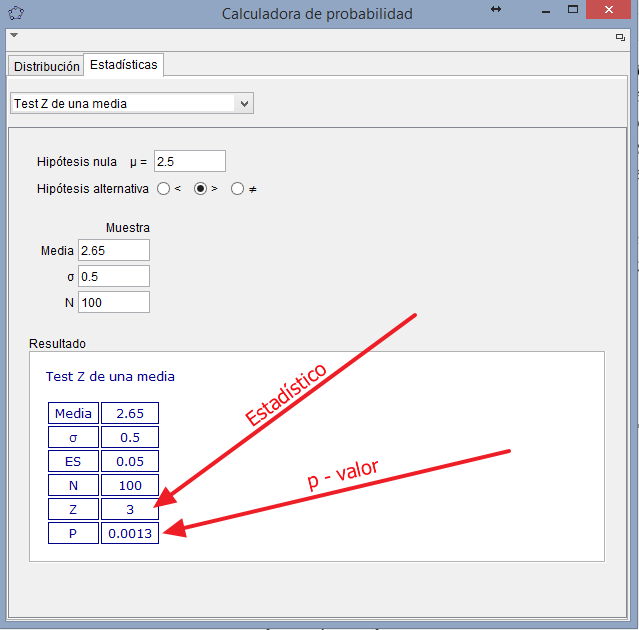
\includegraphics[width=11cm]{../fig/Tut07-11.png}
\end{center}

Inicialmente los campos de esta ventana están vacíos, claro. En esta figura verás el resultado que se obtiene cuando se sustituyen los datos del ejemplo inicial del Capítulo \ref{curso-cap:ContrasteHipotesis} del libro, el Ejemplo \ref{curso-cap07:ejem:CangurosDepresivos03} (pág. \pageref{curso-cap07:ejem:CangurosDepresivos03}). Hemos indicado además, con flechas rojas, los lugares donde aparecen el p-valor y el estadístico del contraste.


\subsection{Potencia y tamaño muestral.}

Vamos a mostrar cómo se llevan a cabo, usando R, las cuentas de los Ejemplos \ref{curso-cap07:ejem:CalculoPotenciaEjemploCanguros} (pág. \pageref{curso-cap07:ejem:CalculoPotenciaEjemploCanguros}) y \ref{curso-cap07:ejem:CalculoPotenciaEjemploCanguros2} (pág. \pageref{curso-cap07:ejem:CalculoPotenciaEjemploCanguros2}) del libro.

En el primero de esos ejemplos hemos visto que para calcular la potencia $1-\beta$ del contraste necesitamos calcular:
\[
    \mbox{potencia}=1-\beta=P\left(Z> z_{\alpha}-\dfrac{\delta}{\dfrac{s}{\sqrt{n}}}\right).
\]
(ver Ecuación \ref{curso-cap07:ecu:EcuacionPotenciaContrasteMediaConZ}, pág. \pageref{curso-cap07:ecu:EcuacionPotenciaContrasteMediaConZ} del libro), donde
    \[\alpha=0.05,\quad \delta=0.1,\quad  s=0.5,\quad  n=100.\]
Para calcular la potencia en R basta por tanto con usar  {\tt pnorm} así:
\begin{knitrout}
\definecolor{shadecolor}{rgb}{0.969, 0.969, 0.969}\color{fgcolor}\begin{kframe}
\begin{alltt}
\hlstd{alpha} \hlkwb{=} \hlnum{0.05}
\hlstd{delta} \hlkwb{=} \hlnum{0.1}
\hlstd{s} \hlkwb{=} \hlnum{0.5}
\hlstd{n} \hlkwb{=} \hlnum{100}

\hlstd{(zAlfa} \hlkwb{=} \hlkwd{qnorm}\hlstd{(}\hlnum{1}\hlopt{-} \hlstd{alfa))}
\end{alltt}
\begin{verbatim}
## [1] 1.6449
\end{verbatim}
\begin{alltt}
\hlstd{(potencia} \hlkwb{=} \hlnum{1} \hlopt{-} \hlkwd{pnorm}\hlstd{(zAlfa} \hlopt{-} \hlstd{delta} \hlopt{/} \hlstd{(s} \hlopt{/} \hlkwd{sqrt}\hlstd{(n)) ))}
\end{alltt}
\begin{verbatim}
## [1] 0.63876
\end{verbatim}
\end{kframe}
\end{knitrout}
como aparece en el Ejemplo \ref{curso-cap07:ejem:CalculoPotenciaEjemploCanguros}. Ten en cuenta que hemos usado {\tt 1 - pnorm} porque estamos calculando la probabilidad de una cola derecha (también puedes usar la opción {\tt lower.tail = FALSE} como hemos visto en el Tutorial05).

El cálculo del tamaño muestral en el Ejemplo \ref{curso-cap07:ejem:CalculoPotenciaEjemploCanguros2} es muy sencillo (ver la Ecuación \ref{curso-cap07:ecu:TamannoMuestralParaPotenciaDadaContrasteMediaConZ}, pág. \ref{curso-cap07:ecu:TamannoMuestralParaPotenciaDadaContrasteMediaConZ} del libro). Vamos a presentar los cálculos completos a partir de los valores del ejemplo, para que te resulte más fácil adaptarlo a otros posibles ejemplos:

\begin{knitrout}
\definecolor{shadecolor}{rgb}{0.969, 0.969, 0.969}\color{fgcolor}\begin{kframe}
\begin{alltt}
\hlstd{potenciaDeseada} \hlkwb{=} \hlnum{0.80}

\hlstd{delta} \hlkwb{=} \hlnum{0.1}

\hlstd{s} \hlkwb{=} \hlnum{0.5}

\hlstd{alfa} \hlkwb{=} \hlnum{0.01}

\hlstd{(zAlfa} \hlkwb{=} \hlkwd{qnorm}\hlstd{(}\hlnum{1}\hlopt{-} \hlstd{alfa))}
\end{alltt}
\begin{verbatim}
## [1] 2.3263
\end{verbatim}
\begin{alltt}
\hlstd{(zPot} \hlkwb{=} \hlkwd{qnorm}\hlstd{(}\hlnum{1} \hlopt{-} \hlstd{potenciaDeseada))}
\end{alltt}
\begin{verbatim}
## [1] -0.84162
\end{verbatim}
\begin{alltt}
\hlstd{(tamannoMuestra} \hlkwb{=}  \hlstd{( (s} \hlopt{/} \hlstd{delta)} \hlopt{*} \hlstd{(zAlfa} \hlopt{-} \hlstd{zPot))}\hlopt{^}\hlnum{2}\hlstd{)}
\end{alltt}
\begin{verbatim}
## [1] 250.9
\end{verbatim}
\end{kframe}
\end{knitrout}

Vamos a posponer parte del estudio de la potencia (y en particular el dibujo de las curvas de potencia), hasta que hayamos podido explorar otros tipos de contrastes de hipótesis, para así poder dar un tratamiento más general a este tipo de cálculos. De momento, aquí tienes un ejercicio para practicar.

\begin{ejercicio}
\label{tut07:ejercicio03}
\begin{enumerate}
  \item[]
  \item Calcula la potencia del contraste que aparece en el apartado 3 del Ejercicio \ref{tut07:ejercicio01} (pág. \pageref{tut07:ejercicio01}), usando $\delta = 0.2$ y $\alpha=0.95$.

  \item Calcula el tamaño muestral necesario para alcanzar una potencia  $0.80$ usando el mismo valor de $\delta$ y $\alpha$.
\end{enumerate}
Soluciones en la página \pageref{tut07:ejercicio03:sol}.
\qed
\end{ejercicio}

\section{Otros tipos de contrastes de hipótesis.}
\label{tut07:sec:OtrosContrastesHipotesis}

El ejemplo inicial del Capítulo \ref{curso-cap:ContrasteHipotesis} del libro, el Ejemplo \ref{curso-cap07:ejem:CangurosDepresivos03} de los canguros depresivos, contiene todos los ingredientes básicos de los contrastes de hipótesis. A medida que avancemos en la Estadística encontraremos muchas variaciones sobre ese tema. Y en esta sección del tutorial vamos a ocuparnos de las primeras de ellas.

\subsection{Los restantes tipos posibles de hipótesis nulas.}
\label{tut07:subsec:RestantesTiposPosiblesHipotesisNulas}

En la Sección \ref{curso-cap07:sec:ContrastesUnilateralesBilaterales} (pág. \pageref{curso-cap07:sec:ContrastesUnilateralesBilaterales}) del libro hemos visto cómo proceder en el caso de un contraste unilateral en el que la hipótesis nula sea de la forma
    \[H_0=\{\mu\geq \mu_0\}\]
y también en el caso de un contraste bilateral  en el que la hipótesis nula sea de la forma
    \[H_0=\{\mu=\mu_0\}.\]
En realidad las cuentas que debemos hacer en estos dos casos son muy  parecidas a las que hemos visto en los ejemplos previos. Vamos a ver sendos ejemplos de cada uno de los tipos de contraste, para que puedas comprobar las similitudes y diferencias entre ellos. Te recomendamos que tengas presentes las figuras que aparecen en la Sección \ref{curso-cap07:sec:ContrastesUnilateralesBilaterales} mientras lees los siguientes Ejemplos.

\subsubsection{Contraste unilateral con $H_0=\{\mu\geq \mu_0\}$.}

Para empezar, vamos a usar este ejemplo, que es un típico ejercicio de libro de texto:

{\em
La inspección de consumo está examinando un envío de latas de conserva, de las que el fabricante afirma que el peso medio son $1000$ gramos. Al examinar una muestra aleatoria de $100$ latas, un inspector obtuvo un peso medio muestral de $998.5$ gramos, con una cuasivarianza muestral de $s^2 = 36.1$ (gramos$^2$). Con esos datos, el inspector se pregunta si el peso medio de las latas será en realidad  menor que el enunciado por el fabricante. Al nivel de confianza $95$\%, ¿qué responderías a la pregunta del inspector? Queremos, además, obtener el p-valor de este contraste.\\
}

En este caso la hipótesis alternativa del inspector es:
\[H_a=\{\mu < \mu_0\},\]
siendo $\mu$ el peso medio real (y desconocido) de las latas, mientras que $\mu_0 = 1000$ gr. es el peso publicitado por el fabricante. Puesto que el tamaño $n = 100$ de la muestra es grande, sabemos que esta cantidad (el estadístico)
\[\dfrac{\bar X - \mu_0}{\dfrac{s}{\sqrt{n}}}\]
se distribuye según la normal $Z\sim N(0,1)$. Para calcular el valor de este estadístico usamos un código muy parecido al del anterior contraste:
\begin{knitrout}
\definecolor{shadecolor}{rgb}{0.969, 0.969, 0.969}\color{fgcolor}\begin{kframe}
\begin{alltt}
\hlstd{mu0} \hlkwb{=} \hlnum{1000}
\hlstd{n} \hlkwb{=} \hlnum{100}
\hlstd{Xbar} \hlkwb{=} \hlnum{998.5}
\hlstd{(s} \hlkwb{=} \hlkwd{sqrt}\hlstd{(}\hlnum{36.1}\hlstd{))}
\end{alltt}
\begin{verbatim}
## [1] 6.0083
\end{verbatim}
\begin{alltt}
\hlstd{(Estadistico} \hlkwb{=} \hlstd{(Xbar} \hlopt{-} \hlstd{mu0)} \hlopt{/} \hlstd{(s} \hlopt{/} \hlkwd{sqrt}\hlstd{(n)))}
\end{alltt}
\begin{verbatim}
## [1] -2.4965
\end{verbatim}
\end{kframe}
\end{knitrout}
Es de esperar que el valor del estadístico sea negativo. Si fuera positivo, querría decir que la media muestral $\bar X$ es mayor que $\mu_0$. Es decir que el peso medio de las latas de la muestra es mayor de lo que afirma el fabricante. Y en tal caso, el inspector no tendría ninguna razón para sospechar de lo que dice el fabricante.

\begin{ejercicio}
\label{tut07:ejercicio04}
\begin{enumerate}
  \item[]
  \item Calcula el valor del estadístico si la media muestral del peso fuera bastante menor de lo que dice el fabricante, por ejemplo $\bar X=990$ gramos.

  \item Calcula ese valor del estadístico si la media muestral del peso fuera prácticamente igual a lo que dice el fabricante, con $\bar X = 999.99$ gramos.

  \item ¿Y cuál sería el valor del estadístico si fuera $\bar X=1005$ gramos?

  \item Haz un dibujo aproximado de la normal estándar $Z$ (no hace falta que sea muy preciso) y sitúa en ese dibujo los valores del estadístico que has calculado en los apartados anteriores. Después responde a estas preguntas: ¿en ese dibujo, dónde están los valores  que nos hacen pensar que $H_a$ puede ser cierta? ¿Y dónde están los valores que nos hacen pensar que $H_0$ puede ser cierta?

  \item ¿Te atreves a calcular el p-valor del contraste? Vamos a ver la respuesta enseguida, pero es bueno que intentes adelantarte para comprobar si estás entendiendo las ideas básicas.
\end{enumerate}
Soluciones en la página \pageref{tut07:ejercicio04:sol}.
\qed
\end{ejercicio}

\quad\\
\vspace{2cm}
\begin{center}
\textcolor{red}{\bf\LARGE ¡No sigas, si no has hecho este ejercicio!}
\end{center}
\vspace{2cm}
\newpage

\subsubsection*{Cálculo del p-valor y la región de rechazo en este caso.}

A la vista de los resultados de este ejercicio y de la discusión de la Sección \ref{curso-cap07:sec:ContrastesUnilateralesBilaterales} del libro (pág. \pageref{curso-cap07:sec:ContrastesUnilateralesBilaterales}), debería estar claro que para calcular el p-valor de este contraste tenemos que usar la cola {\em izquierda} de la distribución normal, porque esa cola la forman los valores favorables a la hipótesis alternativa.
En R, el cálculo sería:
\begin{knitrout}
\definecolor{shadecolor}{rgb}{0.969, 0.969, 0.969}\color{fgcolor}\begin{kframe}
\begin{alltt}
\hlstd{(pValor} \hlkwb{=} \hlkwd{pnorm}\hlstd{(Estadistico))}
\end{alltt}
\begin{verbatim}
## [1] 0.0062707
\end{verbatim}
\end{kframe}
\end{knitrout}
Recuerda que el p-valor indica cómo de improbable le parecen estos datos muestrales a alguien que cree que la hipótesis nula es cierta. En este caso, a alguien que cree que el peso medio de las latas es de $1000$ gramos o más. El resultado que hemos obtenido significa que, si lo que dice el fabricante es cierto, la probabilidad de obtener al azar un lote de $100$ latas con un peso medio $\bar X = 998.5$ es aproximadamente igual a $0.00627$. Parece bastante evidente que el inspector tendría buenas razones para poner bajo sospecha esa afirmación del fabricante.

Naturalmente, el fabricante puede insistir en que ha tenido mala suerte y que los resultados que hemos obtenido pueden ser fruto del azar... Para evitar una discusión improductiva, usamos los niveles de verosimilitud como una forma de zanjar este asunto. Podemos establecer, en los reglamentos de consumo, que los inspectores utilizarán un nivel de significación del contraste 99\%. Es decir $ns = 0.99$, con lo que $\alpha = 0.01$. Y puesto que el p-valor $0.00627$ es  menor que $\alpha$, el inspector puede rechazar la hipótesis nula y sancionar al fabricante por faltar a la verdad sobre el peso de esas latas.

Como ves en este ejemplo, el nivel de significación puede utilizarse para fijar un criterio objetivo, establecido a priori (antes de empezar las inspecciones), que ayuda a todas las partes implicadas al definir ``las reglas del juego''.

¿Cuál es la región de rechazo en este ejemplo, al nivel de confianza del $99$\%? Para calcularla es bueno hacerse la pregunta de esta otra manera. ¿Cuál es el valor del estadístico para el que el p-valor coincide precisamente con $\alpha$? Y el cálculo, en R, sería:
\begin{knitrout}
\definecolor{shadecolor}{rgb}{0.969, 0.969, 0.969}\color{fgcolor}\begin{kframe}
\begin{alltt}
\hlstd{nc} \hlkwb{=} \hlnum{0.99}
\hlstd{(alfa} \hlkwb{=} \hlnum{1} \hlopt{-} \hlstd{nc)}
\end{alltt}
\begin{verbatim}
## [1] 0.01
\end{verbatim}
\begin{alltt}
\hlkwd{qnorm}\hlstd{(alfa)}
\end{alltt}
\begin{verbatim}
## [1] -2.3263
\end{verbatim}
\end{kframe}
\end{knitrout}
Ese valor del estadístico marca la frontera entre los valores que nos llevan a rechazar la hipótesis nula y los valores que no nos hacen rechazarla (recuerda que {\em nunca la aceptamos}).  Cualquier valor del estadístico menor que $-2.326$ nos llevaría a rechazar $H_0$ ¿Por qué menor? Si no ves claro por qué, vuelve a leer este ejemplo y la Sección \ref{curso-cap07:sec:ContrastesUnilateralesBilaterales} del libro hasta que lo entiendas.

\begin{ejercicio}
\label{tut07:ejercicio05}
El valor $-2.326$ que hemos obtenido es un valor tipificado, en la escala $Z$ de la normal estándar.  ¿Cuál es el valor correspondiente en la escala original del problema? Es decir, ¿cuál es peso medio mínimo muestral, en gramos, a partir del cual el inspector rechaza $H_0$? Solución en la página \pageref{tut07:ejercicio05:sol}.
\qed
\end{ejercicio}

\subsubsection{Contraste bilateral con $H_0=\{\mu = \mu_0\}$.}

Vamos a volver a usar el ejemplo de las latas de conservas. Pero ahora vamos a pensar en este mismo problema desde otro punto de vista, desde la perspectiva del fabricante. Es importante entender la diferencia entre su punto de vista y el punto de vista del inspector. Al inspector el único problema que le preocupa es que el peso de las latas pueda ser menor de lo que anuncia el fabricante, porque eso podría suponer un fraude a los consumidores. Si el fabricante decide envasar en cada lata más producto del que anuncia, el inspector no tendrá nada que objetar. En cambio el fabricante tiene que tomar una decisión más complicada. Por un lado, si envasa demasiado poco producto, sabe que el inspector le sancionará. En cambio si, para evitar eso, envasa demasiado producto en cada lata, estará perdiendo dinero. ¿Cuál debe ser entonces su objetivo? Lo razonable es tratar de conseguir que la cantidad de producto envasado se parezca mucho al objetivo marcado $\mu_0=1000$ gramos. Así que el fabricante tratará de controlar el proceso de envasado para ver si se cumple la hipótesis nula (bilateral):
\[ H_0=\{\mu = \mu_0\}.\]
El departamento de control de calidad de la fábrica trabajará para contrastar esta hipótesis frente a la hipótesis alternativa
\[ H_a=\{\mu\neq \mu_0\}.\]
teniendo siempre presente que todas las desviaciones con respecto a $\mu_0$ son malas: si $\mu$  está {\em demasiado} por debajo de $\mu_0$ nos sancionarán, y si $\mu$ está {\em demasiado} por encima de $\mu_0$ estaremos perdiendo dinero.

La clave, en cualquier caso, es la palabra {\em demasiado}. Si los valores del peso envasado son suficientemente parecidos a $\mu_0$ estaremos alcanzando un equilibrio razonable entre ambos problemas.

Vayamos a los datos para ver cómo funciona esto en la práctica. Imagínate que el fabricante, después de la sanción del inspector, ha diseñado un nuevo proceso de envasado, y quiere saber si ese proceso es satisfactorio. Ya sabemos que hay que trabajar a un nivel de confianza del $99\%$ para evitar la sanción del inspector. Así que el fabricante examina una nueva partida de $100$ latas fabricadas con el nuevo sistema de envasado y obtiene una media muestral de $\bar X = 999.7$ gramos, con una cuasivarianza muestral de $s^2 = 20.2$ gramos$^2$.

Para contrastar la hipótesis nula $H_0=\{\mu = 1000\}$ el fabricante empieza por calcular el valor del estadístico:

\begin{knitrout}
\definecolor{shadecolor}{rgb}{0.969, 0.969, 0.969}\color{fgcolor}\begin{kframe}
\begin{alltt}
\hlstd{mu0} \hlkwb{=} \hlnum{1000}
\hlstd{n} \hlkwb{=} \hlnum{100}
\hlstd{Xbar} \hlkwb{=} \hlnum{999.7}
\hlstd{(s} \hlkwb{=} \hlkwd{sqrt}\hlstd{(}\hlnum{20.2}\hlstd{))}
\end{alltt}
\begin{verbatim}
## [1] 4.4944
\end{verbatim}
\begin{alltt}
\hlstd{(Estadistico} \hlkwb{=} \hlkwd{abs}\hlstd{(Xbar} \hlopt{-} \hlstd{mu0)} \hlopt{/} \hlstd{(s} \hlopt{/} \hlkwd{sqrt}\hlstd{(n)))}
\end{alltt}
\begin{verbatim}
## [1] 0.66749
\end{verbatim}
\end{kframe}
\end{knitrout}
{\bf ¡Fíjate en el valor absoluto!} Hemos usado la función {\tt abs} en el estadístico, porque al fabricante le preocupa quedarse corto de peso, pero también le preocupa pasarse.

\begin{ejercicio}
\label{tut07:ejercicio06}
\begin{enumerate}
  \item[]
  \item ¿Cuál sería el valor del estadístico si el peso medio muestral fuera $\bar X= 1000.3$?
  \item ¿Cuál tiene que ser el peso medio muestral para que el estadístico valga $2$? ¿Hay más de una respuesta a esta pregunta?
%  \item Dibuja la normal estándar $Z$ y sitúa en el dibujo esos valores del estadístico. Las preguntas que debes hacerte, como en los anteriores contrastes, es: ¿donde están, en esa figura, los valores favorables a $H_0$? ¿Dónde están los valores favorables a $H_a$?
  \item En este ejemplo de las latas, las dos colas de la distribución normal se pueden identificar, respectivamente, con uno de los problemas que preocupan al fabricante: la sanción de la inspección o el exceso de producto envasado. ¿Qué cola corresponde a cada uno de esos dos problemas?
\end{enumerate}
Soluciones en la página \pageref{tut07:ejercicio06:sol}.
\qed
\end{ejercicio}

\subsubsection*{Cálculo del p-valor y la región de rechazo en este caso.}

El p-valor siempre representa (en cualquier contraste) la probabilidad de obtener un valor del estadístico al menos tan favorable a la hipótesis alternativa como el que hemos obtenido en la muestra. En este caso eso significa que debemos tener en cuenta las dos colas de la distribución normal, porque ambas contienen valores favorables a $H_a$.

Como hemos visto en la Ecuación \ref{curso-cap07:ecu:pValorMediaZBilateral} del libro (pág. \pageref{curso-cap07:ecu:pValorMediaZBilateral}) el p-valor se calcula así a partir del estadístico:
\[
\mbox{p-valor}=
2\cdot P\left(Z > \dfrac{|\bar X-\mu_0|}{\dfrac{s}{\sqrt{n}}}\right)=
2\cdot P\left(Z > \mbox{Estadístico}\right),
\]
lo cual se traduce en este código en R:
\begin{knitrout}
\definecolor{shadecolor}{rgb}{0.969, 0.969, 0.969}\color{fgcolor}\begin{kframe}
\begin{alltt}
\hlstd{(pValor} \hlkwb{=} \hlnum{2} \hlopt{*} \hlstd{(}\hlnum{1} \hlopt{-} \hlkwd{pnorm}\hlstd{(Estadistico)))}
\end{alltt}
\begin{verbatim}
## [1] 0.50446
\end{verbatim}
\end{kframe}
\end{knitrout}

Este p-valor es muy grande (mayor que $1/2$). Y por lo tanto, no rechazamos la hipótesis nula. En términos del ejemplo, este p-valor indica que el fabricante está cumpliendo su objetivo: el valor del peso envasado está suficientemente cerca del objetivo de $\mu_0=1000$ gramos.

\begin{ejercicio}
\label{tut07:ejercicio07}
\begin{enumerate}
  \item[]
  \item ¿Por qué hemos usado {\tt 1 - pnorm} (en lugar de {\tt pnorm}) en este cálculo?

  \item Ahora imagínate de nuevo que eres el inspector y utiliza los mismos datos que el fabricante para contrastar la hipótesis nula unilateral $H_0=\{\mu \geq 1000\}$ a un nivel de significación del $99\%$. ¿Qué p-valor has obtenido? ¿Cuál es la conclusión a la que llega el inspector?



  \item ¿Qué sucede con los p-valores del fabricante y el inspector si $\bar X = 999.1$?



  \item ¿Puede suceder, para unos mismos valores muestrales, que el fabricante no rechace al 99\% la hipótesis nula bilateral $H_0=\{\mu = 1000\}$, pero que el inspector sí rechace la hipótesis nula unilateral $H_0=\{\mu \geq 1000\}$?

\end{enumerate}
Solución en la página \pageref{tut07:ejercicio07:sol}.
\qed
\end{ejercicio}

La región de rechazo, cuando usamos un nivel de significación  $ns = 99\%$, la forman los valores del estadístico  que pertenecen a cualquiera de las dos colas de la distribución $Z$ definidas por el nivel de significación (ver la Figura \ref{curso-cap07:fig:RegionRechazoNormalBilateral} del libro, pág. \pageref{curso-cap07:fig:RegionRechazoNormalBilateral}):
\begin{knitrout}
\definecolor{shadecolor}{rgb}{0.969, 0.969, 0.969}\color{fgcolor}\begin{kframe}
\begin{alltt}
\hlstd{ns} \hlkwb{=} \hlnum{0.99}
\hlstd{(alfa} \hlkwb{=} \hlnum{1} \hlopt{-} \hlstd{ns)}
\end{alltt}
\begin{verbatim}
## [1] 0.01
\end{verbatim}
\begin{alltt}
\hlstd{(alfaMedios} \hlkwb{=} \hlstd{alfa} \hlopt{/} \hlnum{2}\hlstd{)}
\end{alltt}
\begin{verbatim}
## [1] 0.005
\end{verbatim}
\begin{alltt}
\hlstd{(zAlfaMedios} \hlkwb{=} \hlkwd{qnorm}\hlstd{(}\hlnum{1} \hlopt{-} \hlstd{alfaMedios))}
\end{alltt}
\begin{verbatim}
## [1] 2.5758
\end{verbatim}
\end{kframe}
\end{knitrout}
Como indican estos cálculos $z_{\frac{\alpha}{2}}\approx 2.576$. La región de rechazo la forman los valores del estadístico que son mayores que $2.576$ o menores que $-2.576$. Una forma más breve de decir esto es diciendo que son los valores del estadístico {\em cuyo valor absoluto} es mayor que $2.576$.

\subsubsection{Sobre contrastes unilaterales y bilaterales.}
\noindent{\bf Opcional: esta sección puede omitirse en una primera lectura.}

Una lectura atenta de los ejemplos anteriores permite observar que, para un mismo valor de $\mu_0$ y para un nivel de significación dado $ns$, el límite de la región de rechazo de la hipótesis nula del contraste bilateral
\[H_0 = \{\mu = \mu_0\}\]
se sitúa más a la derecha que el límite de la región de rechazo de la hipótesis nula en un contraste unilateral
\[H_0 = \{\mu > \mu_0\}.\]
En definitiva, lo que estamos diciendo se reduce a observar que
\[z_{\alpha} < z_{\frac{\alpha}{2}},\]
ya que esos dos valores definen el límite de las regiones de rechazo. Eso significa que con un valor del estadístico mayor que  $z_{\alpha}$  podemos rechazar $H_0$ en el caso unilateral, mientras que ese mismo valor no permite rechazar $H_0$ en el caso bilateral.

Esta observación tiene una consecuencia que nos parece desafortunada. Ya hemos dicho que en muchas ocasiones la hipótesis nula representa la teoría vigente y  que la hipótesis alternativa representa una teoría nueva que aspira a sustituir a la antigua. Pero en muchas aplicaciones científicas (por ejemplo, y de forma especial, en Ciencias de la Salud) se aplica una forma especial del dicho {\em ``más vale lo malo conocido que lo bueno por conocer''}. Ese principio de precaución hace que, en el contraste de hipótesis, dejemos que la hipótesis nula {\em juegue con ventaja}. Y algunas personas, llevados por un exceso de prudencia, deciden utilizar la región de rechazo del contraste de hipótesis bilateral incluso cuando la hipótesis nula es claramente unilateral. En la práctica, eso equivale a trabajar con $\alpha/2$ en lugar de $\alpha$ y, por lo tanto, cuando esas personas nos dicen que han hecho un contraste de hipótesis al 95\% (con $\alpha=0.05$), en realidad han usado $\alpha/2 = 0.25$  y su nivel de significación es $ns=0.975$. El resultado es, finalmente, que hemos elevado el listón para el rechazo de $H_0$. Pero sería mucho más sencillo, y mucho más claro, si eso es lo que se desea, elevar simplemente el nivel de significación {\bf en el contraste unilateral}.

\subsection{Datos {\em en bruto}.}

En el Tutorial06 hemos establecido una distinción los que llamábamos los {\em problemas del mundo real}, en los que recibimos los datos de la muestra {\em en bruto}, y aquellos otros que llamamos {\em problemas de libro de texto}, en los que el punto de partida son los valores $\bar X$, $n$, $s$, etc. Es importante recordar que esa distinción no es una definición formal. Es simplemente una convención y cada uno de los problemas que nos encontraremos, en los libros o en la vida real, contendrá su propia mezcla peculiar de ambos ingredientes.

Con los contrastes, naturalmente, sucede otro tanto. Los cálculos que hemos realizado hasta ahora, los del Ejemplo \ref{curso-cap07:ejem:CangurosDepresivos03} del libro, son típicos de los {\em problemas de libro de texto}. Si el punto de partida es una muestra {\em en bruto}, tenemos dos opciones. La primera es calcular los valores necesarios (en principio, $\bar X$, $n$, $s$) a partir de la muestra, ya sea a mano o usando un fichero plantilla (en este tutorial te facilitaremos algunos de esos ficheros). La segunda es usar una función como la función {\tt t.test} de R, con la que ya nos hemos encontrado en el Tutorial06. Vamos a dejar para un poco más adelante en el tutorial esta segunda opción, y desarrollaremos ahora la primera.



Para concretar vamos a trabajar con un fichero de datos que hemos cocinado para que imiten lo que sucede en el Ejemplo \ref{curso-cap07:ejem:CangurosDepresivos03}. El fichero es este, que adjuntamos aquí:
\begin{center}
\fichero{../datos/Tut07-Contraste-Media-Z-datos.csv}{
Tut07-Contraste-Media-Z-datos.csv}
\end{center}

Si el punto de partida es un fichero como ese, el plan de trabajo es muy parecido, salvo por el hecho de que primero debes leer los datos (usando {\tt scan} o {\tt read.table}, cada una tiene sus ventajas e inconvenientes) y, una vez leídos, calcular a partir de esos datos los valores de $n$, $\bar X$  y $s$. Por ejemplo con este código:

\begin{knitrout}
\definecolor{shadecolor}{rgb}{0.969, 0.969, 0.969}\color{fgcolor}\begin{kframe}
\begin{alltt}
\hlstd{datos} \hlkwb{=} \hlkwd{read.table}\hlstd{(}\hlkwc{file} \hlstd{=} \hlstr{"../datos/Tut07-Contraste-Media-Z-datos.csv"}\hlstd{)[ ,}\hlnum{1}\hlstd{]}
\hlstd{(n} \hlkwb{=} \hlkwd{length}\hlstd{(datos))}
\end{alltt}
\begin{verbatim}
## [1] 100
\end{verbatim}
\begin{alltt}
\hlstd{(Xbar} \hlkwb{=} \hlkwd{mean}\hlstd{(datos))}
\end{alltt}
\begin{verbatim}
## [1] 2.65
\end{verbatim}
\begin{alltt}
\hlstd{(s} \hlkwb{=} \hlkwd{sd}\hlstd{(datos))}
\end{alltt}
\begin{verbatim}
## [1] 0.5
\end{verbatim}
\end{kframe}
\end{knitrout}
Como ves, los valores coinciden, con la precisión necesaria, con los que aparecen en el Ejemplo \ref{curso-cap07:ejem:CangurosDepresivos03}.

Es {\bf muy importante} entender que el contraste de hipótesis, a partir de este punto, transcurre {\bf exactamente igual que antes.} Calculamos el estadístico
\[\dfrac{\bar X - \mu_0}{\dfrac{s}{\sqrt{n}}}\]
con estos valores (y con $\mu_0$, que procede de la hipótesis nula) y lo usamos para obtener el p-valor o la región de rechazo. Para que quede claro, repetimos el cálculo del p-valor usando exactamente los mismos comandos que vimos en la página \pageref{tut07:subsubsec:CalculoPValorEjemploCanguros}:

\begin{knitrout}
\definecolor{shadecolor}{rgb}{0.969, 0.969, 0.969}\color{fgcolor}\begin{kframe}
\begin{alltt}
\hlstd{mu0} \hlkwb{=} \hlnum{2.5}

\hlstd{(Estadistico} \hlkwb{=} \hlstd{(Xbar} \hlopt{-} \hlstd{mu0)} \hlopt{/} \hlstd{(s} \hlopt{/} \hlkwd{sqrt}\hlstd{(n)))}
\end{alltt}
\begin{verbatim}
## [1] 3
\end{verbatim}
\begin{alltt}
\hlstd{(pValor} \hlkwb{=} \hlnum{1} \hlopt{-} \hlkwd{pnorm}\hlstd{(Estadistico))}
\end{alltt}
\begin{verbatim}
## [1] 0.0013499
\end{verbatim}
\end{kframe}
\end{knitrout}
El resultado es (con toda la precisión que podamos necesitar) el mismo.

Para que puedas practicar esto, aquí tienes un ejercicio.

\begin{ejercicio}
\label{tut07:ejercicio08}

El fichero
\begin{center}
  \fichero{../datos/Tut07-Ejercicio-ContrasteMedia.csv}{Tut07-Ejercicio-ContrasteMedia.csv}
\end{center}
contiene una muestra con cierto número de observaciones de una variable $X$ de tipo normal. Usa esa muestra para contrastar la hipótesis nula:
\[
H_0 = \{\mu \leq 27\}.
\]
Solución en la página \pageref{tut07:ejercicio08:sol}.
\qed
\end{ejercicio}

\subsubsection*{Opcional: ¿Cómo se han cocinado los datos de esta sección?}

En aras de la transparencia, y por si sientes curiosidad, vamos a incluir aquí la receta que hemos usado para cocinar los datos del fichero {\tt Tut07-Contraste-Media-Z-datos.csv} (recuerda que hay que fijar el directorio de trabajo antes de ejecutarlo, para que el fichero {\tt csv} termine almacenado en la carpeta {\sf datos}). El fichero {\tt csv} que vamos a cocinar contiene, usando el lenguaje del Ejemplo \ref{curso-cap07:ejem:CangurosDepresivos03}, las medidas de la altura de los saltos de $100$ canguros depresivos tratados con {\em Pildorín Complex}. Como puedes ver en los resultados del código, la media muestral es $\bar X\approx 2.65$ y la cuasidesviación típica muestral es $s=0.5$. Hemos usado por comodidad {\tt write.table} para escribir esos datos en el fichero {\tt csv}, eliminando los nombres de filas y columnas.
\begin{knitrout}
\definecolor{shadecolor}{rgb}{0.969, 0.969, 0.969}\color{fgcolor}\begin{kframe}
\begin{alltt}
\hlkwd{library}\hlstd{(MASS)}
\hlkwd{set.seed}\hlstd{(}\hlnum{2014}\hlstd{)}
\hlstd{muestra} \hlkwb{=} \hlkwd{c}\hlstd{(}\hlkwd{mvrnorm}\hlstd{(}\hlnum{100}\hlstd{,} \hlkwc{mu} \hlstd{=} \hlnum{2.65}\hlstd{,} \hlkwc{Sigma} \hlstd{=} \hlnum{0.5}\hlopt{^}\hlnum{2}\hlstd{,} \hlkwc{empirical} \hlstd{=} \hlnum{TRUE}\hlstd{))}

\hlkwd{mean}\hlstd{(muestra)}
\end{alltt}
\begin{verbatim}
## [1] 2.65
\end{verbatim}
\begin{alltt}
\hlkwd{sd}\hlstd{(muestra)}
\end{alltt}
\begin{verbatim}
## [1] 0.5
\end{verbatim}
\begin{alltt}
\hlkwd{write.table}\hlstd{(muestra,} \hlkwc{file} \hlstd{=} \hlstr{"../datos/Tut07-Contraste-Media-Z-datos.csv"}\hlstd{,}
        \hlkwc{row.names} \hlstd{=} \hlnum{FALSE}\hlstd{,} \hlkwc{col.names}\hlstd{=}\hlnum{FALSE} \hlstd{)}
\end{alltt}
\end{kframe}
\end{knitrout}
Si tienes dudas sobre el funcionamiento de {\tt mvrnorm} puedes volver a la página \pageref{tut06-tut06:subsubsec:CocinandoMuestras} del Tutorial06.

%Fíjate además en que al cocinar la muestra hemos elegido que la cuasidesviación típica muestral fuese $s \approx 0.5$. Pero en el Ejemplo \ref{curso-cap07:ejem:CangurosDepresivos03} no hemos usado  $s$ sino el valor poblacional $\sigma$, que se suponía conocido. Así que en realidad no era necesario ajustar el valor de $s$ al cocinar la muestra: no lo íbamos a usar en cualquier caso. Lo hemos hecho para mantener, no obstante, el ``realismo'' de los datos.


%muy especialmente el Ejemplo \ref{curso-cap07:ejem:ErrorTipicoContrastesHipotesis} (pág. \pageref{curso-cap07:ejem:ErrorTipicoContrastesHipotesis}).  Y para hacerlo, le proponemos un par de ejercicios.

\subsection{Contrastes para $\mu$ en poblaciones normales con muestras pequeñas.}
\label{tut07:subsec:ContrastesMuestrasPequennas}

En la Sección \ref{curso-cap07:sec:contrasteHipotesisMediaMuestrasPequennas} del libro (pág. \pageref{curso-cap07:sec:contrasteHipotesisMediaMuestrasPequennas}) hemos extendido las ideas del contraste de hipótesis al caso de la media de poblaciones normales usando muestras pequeñas. La única novedad con respecto a lo que ya hemos visto es el uso de la $t$ de Student en lugar de la distribución normal. Así que vamos a limitarnos a proponerte una serie de ejercicios para que te ejercites con ese tipo de problemas.

\begin{ejercicio}
\label{tut07:ejercicio09}
En los dos casos debes escribir la hipótesis nula, la hipótesis alternativa, calcular el estadístico,  el p-valor y la región de rechazo al $95\%$.
\begin{enumerate}
  \item En un experimento para medir el tiempo de reacción de las personas se les muestra a los sujetos un círculo de color en la pantalla del ordenador. Cuando el círculo cambia de color, el sujeto debe pulsar la barra de espacio del teclado tan rápido como pueda. En una sesión concreta del experimento, se midieron estos tiempos de reacción de un sujeto (en segundos).
      \[0.316,\quad 0.295,\quad 0.304,\quad 0.263,\quad 0.25\]
      El experimentador sospecha que el tiempo de reacción medio de este sujeto está por debajo de los 0.29 segundos. ¿Confirman estos datos sus sospechas?
  \item Un laboratorio farmacéutico prepara comprimidos que deben contener una dosis de 500mg de cierto principio activo. El sistema de control de calidad del laboratorio ha tomado una muestra de 15 comprimidos para comprobar si la dosis se ajusta a lo esperado. Los valores medidos, en miligramos, son:
        \[
491,\,\,\, 503,\,\,\, 492,\,\,\, 502,\,\,\, 490,\,\,\, 500,\,\,\, 500,\,\,\, 501,\,\,\, 501,\,\,\, 501,\,\,\, 505,\,\,\, 491,\,\,\, 501,\,\,\, 493,\,\,\, 492
        \]
      Utiliza estos valores para comprobar si la dosis es la deseada.
\end{enumerate}
Soluciones en la página \pageref{tut07:ejercicio09:sol}.
\qed
\end{ejercicio}


\subsection{Contrastes para $\sigma^2$ en poblaciones normales.}
\label{tut07:subsec:ContrastesSigma2}

Para cerrar el muestrario de contrastes de hipótesis que hemos visto en el Capítulo \ref{curso-cap:ContrasteHipotesis}, vamos a dedicar esta breve sección a los contrastes de hipótesis sobre la varianza (o desviación típica) de una población normal, que hemos discutido en la Sección \ref{curso-cap07:sec:contrasteHipotesisSigma2} del libro (pág. \pageref{curso-cap07:sec:contrasteHipotesisSigma2}). En concreto, vamos a realizar con los cálculos necesarios para el Ejemplo
\ref{curso-cap07:ejem:ContrasteVarianzaLatasConserva} del libro (pág.
\pageref{curso-cap07:ejem:ContrasteVarianzaLatasConserva}). En ese ejemplo queremos contrastar la hipótesis nula
\[H_0=\{\sigma\leq \sigma_0\},\]
donde $\sigma_0=0.2$, y tenemos:
\begin{knitrout}
\definecolor{shadecolor}{rgb}{0.969, 0.969, 0.969}\color{fgcolor}\begin{kframe}
\begin{alltt}
\hlstd{sigma0} \hlkwb{=} \hlnum{0.2}
\hlstd{n} \hlkwb{=} \hlnum{15}
\hlstd{s} \hlkwb{=} \hlnum{0.24}
\end{alltt}
\end{kframe}
\end{knitrout}
A partir de estos valores calculamos el estadístico y los grados de libertad:
\begin{knitrout}
\definecolor{shadecolor}{rgb}{0.969, 0.969, 0.969}\color{fgcolor}\begin{kframe}
\begin{alltt}
\hlstd{(Y} \hlkwb{=} \hlstd{(n}\hlopt{-}\hlnum{1}\hlstd{)} \hlopt{*} \hlstd{s}\hlopt{^}\hlnum{2} \hlopt{/} \hlstd{sigma0}\hlopt{^}\hlnum{2}\hlstd{)}
\end{alltt}
\begin{verbatim}
## [1] 20.16
\end{verbatim}
\begin{alltt}
\hlstd{k} \hlkwb{=} \hlstd{n} \hlopt{-} \hlnum{1}
\end{alltt}
\end{kframe}
\end{knitrout}
y obtenemos el p-valor mediante
\begin{knitrout}
\definecolor{shadecolor}{rgb}{0.969, 0.969, 0.969}\color{fgcolor}\begin{kframe}
\begin{alltt}
\hlstd{(pvalor} \hlkwb{=} \hlnum{1} \hlopt{-} \hlkwd{pchisq}\hlstd{(Y,} \hlkwc{df} \hlstd{= k))}
\end{alltt}
\begin{verbatim}
## [1] 0.12518
\end{verbatim}
\end{kframe}
\end{knitrout}
y, como indicábamos en el libro, este p-valor es bastante grande, así que no rechazamos $H_0$.

Por supuesto, también es posible trabajar a partir de una muestra en bruto.
Para que puedas practicarlo te proponemos un ejercicio:

\begin{ejercicio}
\label{tut07:ejercicio10}
Supongamos que $X$ es una variable normal y que $\sigma$ es la desviación típica de $X$. Queremos contrastar la hipótesis alternativa
\[H_a=\{\sigma \neq 3.7\}\]

Para ello hemos tomado una muestra aleatoria que encontrarás en el fichero
\begin{center}
  \fichero{../datos/Tut07-Ejercicio-ContrasteVarianza.csv}{Tut07-Ejercicio-ContrasteVarianza.csv}
\end{center}
Calcula el p-valor del contraste (recuerda que es bilateral). Solución en la página \pageref{tut07:ejercicio10:sol}.
\qed
\end{ejercicio}


\subsection{Ficheros {\em plantilla} de comandos R para estos contrastes.}
\label{tut07:subsec:FicherosPlantillaRContrastes}

La experiencia que has acumulado en las secciones previas de este tutorial debe servir para ayudarte a entender las decisiones que hay que tomar en un contraste de hipótesis sobre la media o la varianza. Es sencillo, entonces, con un poco de cuidado, automatizar ese proceso de toma de decisiones, para obtener un programa en R que a partir de los datos del problema calcule el p-valor y la región de rechazo del contraste.

En la Tabla \ref{tut07:tabla:FicherosPlantillaRContrastes} (pág. \pageref{tut07:tabla:FicherosPlantillaRContrastes}) encontrarás una lista con varios de esos programas, que cubren todas las situaciones que puedes encontrarte al realizar un contraste como los que hemos descrito en el Capítulo \ref{curso-cap:ContrasteHipotesis} del libro.   Como hicimos en el caso de los intervalos de confianza, distinguimos entre el caso en el que disponemos de los estimadores de la muestra ($n$, $\bar X$, $s$) y el caso en el que disponemos de todos los datos de la muestra (muestra ``en bruto'').  Todos los ficheros incluyen, al principio, un bloque de comandos en el que debes introducir los datos del problema. Si dispones de datos en bruto, ya sea en forma de vector o de fichero {\tt csv} tendrás que descomentar algunas líneas para usarlas. Y, en cualquier caso, {\bf siempre deberás indicar el tipo de contraste} que quieres realizar, mediante un código numérico (del $1$ al $3$) que identifica los contrastes unilaterales o bilaterales posibles. Tienes instrucciones detalladas en los comentarios de los ficheros, así que lee esas instrucciones detenidamente
antes de usar estos ficheros.

\begin{table}[b!]
\fbox{
\begin{minipage}{15cm}
    \begin{itemize}
      \item Contrastes para la media en poblaciones normales o con muestras suficientemente grandes.
        \begin{itemize}

          \item Muestra grande o el caso de $\sigma$ conocida.

                \begin{itemize}

                  \item Estadísticos de la muestra:
                    \fichero{./code/Tut07-Contraste-Media-UsandoZ.R}{Tut07-Contraste-Media-UsandoZ.R}

                  \item Datos en bruto:
                    \fichero{./code/Tut07-Contraste-Media-UsandoZ-DatosEnBruto.R}{Tut07-Contraste-Media-UsandoZ-DatosEnBruto.R}

                \end{itemize}

          \item Muestra pequeña.

                \begin{itemize}

                  \item Estadísticos de la muestra:
                    \fichero{./code/Tut07-Contraste-Media-UsandoT.R}{Tut07-Contraste-Media-UsandoT.R}

                  \item Datos en bruto:
                    \fichero{./code/Tut07-Contraste-Media-UsandoT-DatosEnBruto.R}{Tut07-Contraste-Media-UsandoT-DatosEnBruto.R}

                \end{itemize}

        \end{itemize}

      \item Contrastes para la varianza o desviación típica  en poblaciones          normales.

                \begin{itemize}\item[]\begin{itemize}

                  \item Estadísticos de la muestra:
                    \fichero{./code/Tut07-Contraste-Varianza-PobNormal-Estadisticos.R}{Tut07-Contraste-Varianza-PobNormal-Estadisticos.R}

                  \item Datos en bruto:
                    \fichero{./code/Tut07-Contraste-Varianza-PobNormal-DatosEnBruto.R}{Tut07-Contraste-Varianza-PobNormal-DatosEnBruto.R}

                \end{itemize}\end{itemize}

    \end{itemize}
\end{minipage}
}
  \caption{Ficheros plantilla de R para contrastes de hipótesis}
  \label{tut07:tabla:FicherosPlantillaRContrastes}
\hrule
\end{table}

Para practicar el uso de estos ficheros, aquí tienes unos cuantos ejercicios.

\begin{ejercicio}
\label{tut07:ejercicio11}
\label{tut07:subsubsec:EjerciciosContrasteHipotesis}
En todos los casos, es tarea tuya seleccionar el fichero plantilla adecuado para realizar el contraste.
\begin{enumerate}

    \item Comprueba los cálculos del Ejemplo \ref{curso-cap07:ejem:CangurosDepresivos03}, pág. \pageref{curso-cap07:ejem:CangurosDepresivos03} del libro.

    \item Utiliza los datos del fichero \fichero{../datos/Tut07-Ejercicios-Contrastes-01.csv}{Tut07-Ejercicios-Contrastes-01.csv} para contrastar la hipótesis nula $H_0=\{\mu\leq \mu_0\}$, siendo $\mu_0=27$. Usa un nivel de significación del 95\%. Primero puedes suponer que $\sigma$ es conocida, y vale $1$. Después repite el contraste suponiendo que no conocemos $\sigma$. ¿Llegas a la misma conclusión?

    \item Comprueba los cálculos del Ejemplo \ref{curso-cap07:ejem:ContrasteMediaMuestrasPequennas}, página \pageref{curso-cap07:ejem:ContrasteMediaMuestrasPequennas} del libro. Ten en cuenta que se hacen dos contrastes en ese ejemplo.

    \item Utiliza los datos del fichero \fichero{../datos/Tut07-Ejercicios-Contrastes-02.csv}{Tut07-Ejercicios-Contrastes-02.csv} para contrastar la hipótesis nula $H_0=\{\mu=\mu_0\}$, siendo $\mu_0=2.2$. Usa un nivel de significación del 95\%.

    \item Comprueba los cálculos del Ejemplo \ref{curso-cap07:ejem:ContrasteVarianzaLatasConserva},
      página \pageref{curso-cap07:ejem:ContrasteVarianzaLatasConserva} del libro.

    \item Usando los datos del fichero \fichero{../datos/Tut07-Ejercicios-Contrastes-03.csv}{Tut07-Ejercicios-Contrastes-03.csv}, contrasta (al 95\%) la hipótesis nula $H_0={\sigma\geq 0.56}$.
\end{enumerate}
%Soluciones en la página \pageref{tut07:ejercicio11:sol}.
\qed
\end{ejercicio}

\subsection{La función {\tt t.test} de R (y sus parientes)}

Vamos a ver como usar la función {\tt t.test} de R (que ya conocimos en la página \pageref{tut06-tut06:subsubsec:CocinandoMuestras} del Tutorial06) para realizar un contraste de hipótesis sobre la media.

Una compañía ferroviaria canadiense afirma que sus trenes de mercancías no bloquean los pasos a
nivel durante más de 8 minutos, en promedio. Una muestra aleatoria de 10 tiempos de bloqueo dio
como resultado estos valores (en minutos):

\begin{center}
{\tt 10.1, 9.5, 6.5, 8.0, 8.8, 12,  7.2, 10.5, 8.2, 9.3}
\end{center}

Empezamos por observar que en este caso tenemos todos los valores de la muestra. Si llamamos $\mu$ al tiempo medio de bloqueo, queremos usar estos valores para contrastar la hipótesis nula:
\[H_0=\{ \mu \leq \mu_0=8 \}\]
Y naturalmente la hipótesis alternativa es:
\[H_a=\{ \mu > \mu_0=8 \}\]
Vamos a fijar un nivel de significación del 95\%, es decir, $\alpha=0.05$. Puesto que se trata de una muestra pequeña $(n=10)$, usaremos la distribución $t$ de Student para el cálculo del p-valor.

\begin{ejercicio}
\label{tut07:ejercicio12}
Haz primero los cálculos del contraste utilizando el fichero
\begin{center}
{\tt Tut07-Contraste-Media-UsandoT-DatosEnBruto.R,}
\end{center}
sin recurrir a {\tt t.test}. Solución en la página \pageref{tut07:ejercicio12:sol}.
\qed
\end{ejercicio}

Este ejercicio muestra que, con un nivel de significación 0.05 (mayor que el p-valor), tenemos evidencia empírica para rechazar la hipótesis nula y concluir que los trenes bloquean el paso a nivel más tiempo del que dice la empresa. Veamos ahora como hacer este mismo contraste usando {\tt t.test}:

\begin{knitrout}
\definecolor{shadecolor}{rgb}{0.969, 0.969, 0.969}\color{fgcolor}\begin{kframe}
\begin{alltt}
\hlstd{datos}\hlkwb{=}\hlkwd{c}\hlstd{(}\hlnum{10.1}\hlstd{,} \hlnum{9.5}\hlstd{,} \hlnum{6.5}\hlstd{,} \hlnum{8.0}\hlstd{,} \hlnum{8.8}\hlstd{,} \hlnum{12}\hlstd{,} \hlnum{7.2}\hlstd{,} \hlnum{10.5}\hlstd{,} \hlnum{8.2}\hlstd{,} \hlnum{9.3}\hlstd{)}
\hlstd{mu0}\hlkwb{=}\hlnum{8}
\hlstd{(contraste} \hlkwb{=} \hlkwd{t.test}\hlstd{(datos,}\hlkwc{mu}\hlstd{=mu0,}\hlkwc{alternative}\hlstd{=}\hlstr{"greater"}\hlstd{,}\hlkwc{conf.level} \hlstd{=} \hlnum{0.95}\hlstd{))}
\end{alltt}
\begin{verbatim}
## 
## 	One Sample t-test
## 
## data:  datos
## t = 1.96, df = 9, p-value = 0.041
## alternative hypothesis: true mean is greater than 8
## 95 percent confidence interval:
##  8.064   Inf
## sample estimates:
## mean of x 
##      9.01
\end{verbatim}
\end{kframe}
\end{knitrout}

Como se ve, aparte del vector de datos, le hemos indicado a R el valor de $\mu_0$ y, mediante las
opciones  {\tt alternative = c("greater")} y {\tt conf.level = 0.95}, hemos seleccionado un contraste de cola derecha ({\tt greater}) y el nivel de significación deseado (mediante {\tt conf.level}, R usa aquí la misma terminología que para los intervalos de confianza, en lugar de hablar de niveles de significación).  Si quieres hacer un contraste de otro tipo, con la cola izquierda o bilateral, debes usar {\tt alternative = c("less")} o bien {\tt alternative = c("two.sided")}, respectivamente.

La respuesta de R contiene tanto el valor del estadístico de contraste en la forma {\tt t =}1.95712 , como el p-valor, en {\tt p-value =}0.04101. Además, para que la interpretación del resultado sea más fácil, y para que podamos comprobar que estamos haciendo lo que deseamos, R describe la hipótesis alternativa del contraste. Como subproducto se obtiene lo que R llama un intervalo de confianza. Ten en cuenta, en cualquier caso que nosotros no hemos visto en el curso este caso de los intervalos de confianza unilaterales.

\subsubsection{La librería {\tt TeachingDemos}. Contrastes para $\mu$ y $\sigma$}
\label{tut07:subsubsec:TeachingDemos}

Después de conocer {\tt t.test} seguramente te estarás preguntado ¿y no hay algo equivalente para hacer un contraste para la media con la $Z$, la normal estándar?  Lo cierto es que esos contrastes $Z$ son casi exclusivamente ``ejemplos de libro de texto'', que no se usan en las aplicaciones reales. Y no se incluyen en R por defecto (¿hemos dicho ya que R no se diseñó pensando en la enseñanza?). Pero eso no significa que no estén disponibles. Basta con cargar una librería, cuyo revelador nombre es {\tt TeachingDemos} (tendrás que instalarla previamente, claro, si no lo  has hecho previamente), y con eso ya tenemos disponible la función {\tt z.test}, con la que podemos hacer esos contrastes.


Vamos a usar esa función {\tt z.test} para rehacer el apartado 2 del Ejercicio \ref{tut07:ejercicio11} de la página \pageref{tut07:ejercicio11} de este tutorial. Recuerda que debes seleccionar como directorio de trabajo aquel que contiene la carpeta {\tt datos}, que a su vez debe contener el fichero:
\begin{center}
{\tt Tut07-Contraste-Media-UsandoT-datos.csv}
\end{center}
Una vez hecho esto, vamos a mostrar el código que permite realizar el contraste (se muestra también la salida), y a continuación lo comentaremos:
\begin{knitrout}
\definecolor{shadecolor}{rgb}{0.969, 0.969, 0.969}\color{fgcolor}\begin{kframe}
\begin{alltt}
\hlkwd{library}\hlstd{(TeachingDemos)}
\hlstd{muestra} \hlkwb{=} \hlkwd{read.table}\hlstd{(}\hlkwc{file}\hlstd{=}\hlstr{"../datos/Tut07-Contraste-Media-UsandoZ-datos.csv"}\hlstd{,}\hlkwc{sep}\hlstd{=}\hlstr{" "}\hlstd{,}\hlkwc{dec}\hlstd{=}\hlstr{"."}\hlstd{)[,}\hlnum{1}\hlstd{]}
\hlkwd{mean}\hlstd{(muestra)}
\end{alltt}
\begin{verbatim}
## [1] 27.1
\end{verbatim}
\begin{alltt}
\hlstd{(contraste} \hlkwb{=} \hlkwd{z.test}\hlstd{(muestra,} \hlkwc{mu} \hlstd{=} \hlnum{27}\hlstd{,} \hlkwc{stdev} \hlstd{=} \hlnum{1}\hlstd{,}
  \hlkwc{alternative}\hlstd{=}\hlstr{"greater"}\hlstd{,} \hlkwc{conf.level} \hlstd{=} \hlnum{0.95}\hlstd{))}
\end{alltt}
\begin{verbatim}
## 
## 	One Sample z-test
## 
## data:  muestra
## z = 1.73, n = 300.0000, Std. Dev. = 1.0000, Std. Dev. of the
## sample mean = 0.0577, p-value = 0.042
## alternative hypothesis: true mean is greater than 27
## 95 percent confidence interval:
##  27.005    Inf
## sample estimates:
## mean of muestra 
##            27.1
\end{verbatim}
\end{kframe}
\end{knitrout}

Puedes ver que el p-valor (que es aproximadamente 0.04163) permite rechazar $H_0$, pero po rmuy poco margen. Como ves, la llamada a la función {\tt z.test} incluye el argumento {\tt stdev=1}, que representa el valor de $\sigma$, la desviación típica de la población {\bf que en este caso se supone conocida} (ya sabes que eso sucede muy pocas veces en la práctica). El argumento {\tt mu=7} se usa para indicarle a R el valor que nosotros llamamos $\mu_0$ en los contrastes. Enseguida volveremos con la segunda parte de este ejercicio, en la que se supone que $\sigma$ es desconocida. Pero antes, vamos a hacernos algunas preguntas sobre este primer cálculo, en forma de ejercicios.

\begin{ejercicio}
\label{tut07:ejercicio13}
\begin{enumerate}
  \item[]
  \item {\em En la salida de {\tt z.test} para este ejemplo se incluye un {\em intervalo de confianza unilateral}, que es $(27.00503, \ensuremath{\infty{}})$. ¿Qué relación hay entre este intervalo y la región de rechazo para este tipo de contrastes, que aparece en la Ecuación \ref{curso-cap07:ecu:RegionRechazoMediaZColaDerecha} (pág. \pageref{curso-cap07:ecu:RegionRechazoMediaZColaDerecha}) del curso? }

  \item ¿Qué ocurre si haces este contraste usando la $t$ de Student (con el fichero adecuado de la Tabla  \ref{tut07:tabla:FicherosPlantillaRContrastes}, pág. \pageref{tut07:tabla:FicherosPlantillaRContrastes})? ¿Qué p-valor obtienes?

\end{enumerate}

%Soluciones en la página \pageref{tut07:ejercicio13:sol}.
\qed
\end{ejercicio}


Volvamos a la segunda parte del Ejercicio 2 de la página \pageref{tut07:subsubsec:EjerciciosContrasteHipotesis}. Ahora ya no suponemos $\sigma$ conocido y por esa razón tenemos que cambiar la forma en la que llamamos a {\tt z.test}.  La nueva versión es esta:

\begin{knitrout}
\definecolor{shadecolor}{rgb}{0.969, 0.969, 0.969}\color{fgcolor}\begin{kframe}
\begin{alltt}
\hlkwd{z.test}\hlstd{(muestra,} \hlkwc{mu} \hlstd{=} \hlnum{27}\hlstd{,} \hlkwc{sd} \hlstd{=} \hlkwd{sd}\hlstd{(muestra),}
  \hlkwc{alternative} \hlstd{=} \hlstr{"greater"}\hlstd{,} \hlkwc{conf.level} \hlstd{=} \hlnum{0.95}\hlstd{)}
\end{alltt}
\begin{verbatim}
## 
## 	One Sample z-test
## 
## data:  muestra
## z = 2.17, n = 300.0000, Std. Dev. = 0.8000, Std. Dev. of the
## sample mean = 0.0462, p-value = 0.015
## alternative hypothesis: true mean is greater than 27
## 95 percent confidence interval:
##  27.024    Inf
## sample estimates:
## mean of muestra 
##            27.1
\end{verbatim}
\end{kframe}
\end{knitrout}

en la que, como puedes ver, hemos cambiado el argumento {\tt stdev = 1.5} por {\tt sd = sd(muestra)}, indicándole a la R que utilice la cuasidesviación típica muestral en lugar de $\sigma$. El p-valor es ligeramente distinto, claro, y ahora nos permite rechazar $H_0$ con más claridad.

Como hemos visto, la función {\tt z.test} trabaja a partir de un vector de datos. Si lo que tenemos son los estimadores (o descriptores) de una muestra, como $n$, $\bar X$, $s$, entonces debemos utilizar el método que vimos en la página \pageref{tut06-tut06:subsubsec:CocinandoMuestras} del Tutorial06, basado en la función {\tt mvrnorm}.


Para terminar con esta visita a la librería {\tt TeachingDemos}, vamos a presentar la función {\tt sigma.test} que, como su nombre sugiere, sirve para realizar un contraste de hipótesis sobre la desviación típica $\sigma$ de una población normal. En el siguiente fragmento de código R hemos usado esta librería para obtener el contraste que se pedía en el apartado $6$ del Ejercicio \ref{tut07:ejercicio11}  (pág. \pageref{tut07:ejercicio11}).

\begin{knitrout}
\definecolor{shadecolor}{rgb}{0.969, 0.969, 0.969}\color{fgcolor}\begin{kframe}
\begin{alltt}
\hlstd{muestra} \hlkwb{=} \hlkwd{read.table}\hlstd{(}\hlkwc{file}\hlstd{=}\hlstr{"../datos/Tut07-Contraste-Varianza-datos.csv"}\hlstd{,}\hlkwc{sep}\hlstd{=}\hlstr{" "}\hlstd{,}\hlkwc{dec}\hlstd{=}\hlstr{"."}\hlstd{)[ ,}\hlnum{1}\hlstd{]}
\hlkwd{sigma.test}\hlstd{(muestra,}\hlkwc{sigma}\hlstd{=}\hlnum{0.56}\hlstd{,}\hlkwc{alternative}\hlstd{=}\hlstr{"less"}\hlstd{,}\hlkwc{conf.level}\hlstd{=}\hlnum{0.95}\hlstd{)}
\end{alltt}
\begin{verbatim}
## 
## 	One sample Chi-squared test for variance
## 
## data:  muestra
## X-squared = 214, df = 249, p-value = 0.055
## alternative hypothesis: true variance is less than 0.3136
## 95 percent confidence interval:
##  0.00000 0.31506
## sample estimates:
## var of muestra 
##         0.2701
\end{verbatim}
\end{kframe}
\end{knitrout}

El modo de usar de la función {\tt sigma.test}, como ves, es muy fácil de entender. La única precaución que debemos tener es la de utilizar el argumento {\tt sigma=} cuando la hipótesis está formulada en términos de la desviación típica, mientras que se usa {\tt sigmasq=} cuando es la varianza $\sigma_0^2$ la que aparece en las hipótesis del contraste. Por ejemplo, se obtiene exactamente el mismo resultado de antes si se usa esta otra versión:

\begin{knitrout}
\definecolor{shadecolor}{rgb}{0.969, 0.969, 0.969}\color{fgcolor}\begin{kframe}
\begin{alltt}
\hlkwd{sigma.test}\hlstd{(muestra,}\hlkwc{sigmasq}\hlstd{=}\hlnum{0.56}\hlopt{^}\hlnum{2}\hlstd{,}\hlkwc{alternative}\hlstd{=}\hlstr{"less"}\hlstd{,}\hlkwc{conf.level}\hlstd{=}\hlnum{0.95}\hlstd{)}
\end{alltt}
\end{kframe}
\end{knitrout}


\begin{ejercicio}
\label{tut07:ejercicio14}
\begin{enumerate}
  \item[]
  \item Ejecuta ese comando y comprueba que la respuesta es la misma.

  \item Para realizar un contraste sobre la media, en el Ejercicio \ref{tut07:subsubsec:EjerciciosContrasteHipotesis} (pág. )  hemos supuesto primero que $\sigma=1$ era conocido, y luego hemos usado el valor de $s$ obtenido en la muestra. Usa la función {\tt sigma.test} para contrastar la hipótesis $H_a=\{\sigma \neq 1\}$ al 95\%.

\end{enumerate}

%Soluciones en la página \pageref{tut07:ejercicio14:sol}.
\qed
\end{ejercicio}




\subsubsection{La librería {\tt asbio}}\label{tut07:subsubsec:asbio}

En la Sección \ref{tut06-tut06:sec:LibreriaAsbio} del Tutorial06 también aprendimos a usar la librería {\tt asbio} para obtener intervalos de confianza. Esa librería incluye, además, funciones para algunos de los contrastes de hipótesis que estamos viendo. Concretamente, se incluyen entre otras las dos funciones:

\begin{itemize}
  \item {\tt one.sample.z}, para contrastes sobre $\mu$ usando $Z$.
  \item {\tt one.sample.t}, para contrastes sobre $\mu$ usando la $t$ de Student.
\end{itemize}

Una ventaja de estas funciones de {\tt asbio} es que son capaces de funcionar tanto con datos en bruto, como con los valores de $n$, $\bar X$ y $s$. Vamos a dejar que el lector explore esas dos funciones por si mismo:

\begin{ejercicio}
\label{tut07:ejercicio15}
\begin{enumerate}
  \item[]
  \item Lee la descripción de estas dos funciones en la ayuda de la librería {\tt asbio}. Si estás en RStudio, ve al panel {\em Packages} y haz clic sobre el nombre de la librería {\tt asbio}.
  \item Úsalas para volver a hacer algunos de los Ejercicios previos y comprueba que obtienes los mismos resultados.
\end{enumerate}
%Soluciones en la página \pageref{tut07:ejercicio15:sol}.
\qed
\end{ejercicio}


\subsection{Contrastes de hipótesis para $\mu$ y $\sigma$ (una población normal) usando otros programas}

\subsubsection*{Hojas de cálculo: desaconsejamos su uso}

Empecemos por lo más fácil. Calc no incluye funciones para realizar los contrastes que hemos visto, no en el sentido de que sean mínimamente comparables con lo que podemos hacer en R. Existen dos funciones, {\tt PRUEBA.T} y {\tt PRUEBA.Z}, pero sólo las mencionamos para recomendar al lector que no gaste demasiado tiempo tratando de aprender a usarlas: son muy limitadas. Las últimas versiones de otras hojas de cálculo más sofisticadas, como Excel en Microsoft Office 2013, incluyen algunas funciones adicionales para estos contrastes. Pero estas tareas se realizan con mucha más facilidad usando software estadístico como R.

\subsubsection*{Wolfram Alpha.}

Por contra, Wolfram Alpha es capaz de realizar muchos de estos contrastes, con una sintaxis bastante sencilla. Prueba a utilizar el comando:

{\tt z.test for population mean}

y llegarás a un cuadro de diálogo en el que puedes introducir los valores concretos de la muestra, como puedes ver en la Figura \ref{tut07:fig:contrasteHipotesisMediaWolframAlpha} (pág. \pageref{tut07:fig:contrasteHipotesisMediaWolframAlpha}), en la que hemos usado los valores del Ejemplo \ref{curso-cap07:ejem:CangurosDepresivos03} del libro.


Por supuesto, también existe una interfaz similar para el contraste basado en la $t$ de Student, que encontrarás usando:

{\tt t-test for population mean}

No he encontrado información sobre una implementación equivalente para el contraste de hipótesis sobre $\sigma$, usando $\chi^2$. Naturalmente, es posible usar Wolfram Alpha para calcular la probabilidad de una cola de la distribución $\chi^2$, como en este ejemplo donde el comando:

{\tt P[X>23] for X~chi-squared with 20 dof}

permite calcular la probabilidad $P(\chi^2_{20}>23)$, como se ve en la Figura  \ref{tut07:fig:ProbabilidadChiCuadradoWolframAlpha} (pág. \pageref{tut07:fig:ProbabilidadChiCuadradoWolframAlpha}). A partir de aquí, el cálculo de p-valores es fácil, aunque más laborioso, claro.

%\newpage

\begin{figure}[h!]
\begin{center}
    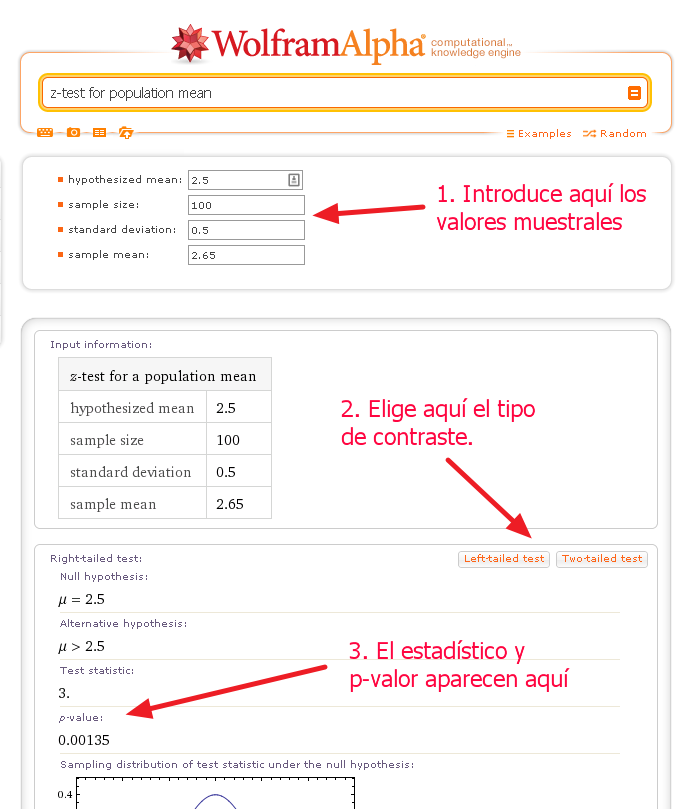
\includegraphics[width=11cm]{../fig/Tut07-02.png}
\end{center}
\caption{Wolfram Alpha para un contraste de hipótesis sobre la media.}
\label{tut07:fig:contrasteHipotesisMediaWolframAlpha}
\end{figure}

\begin{figure}[h!]
\begin{center}
    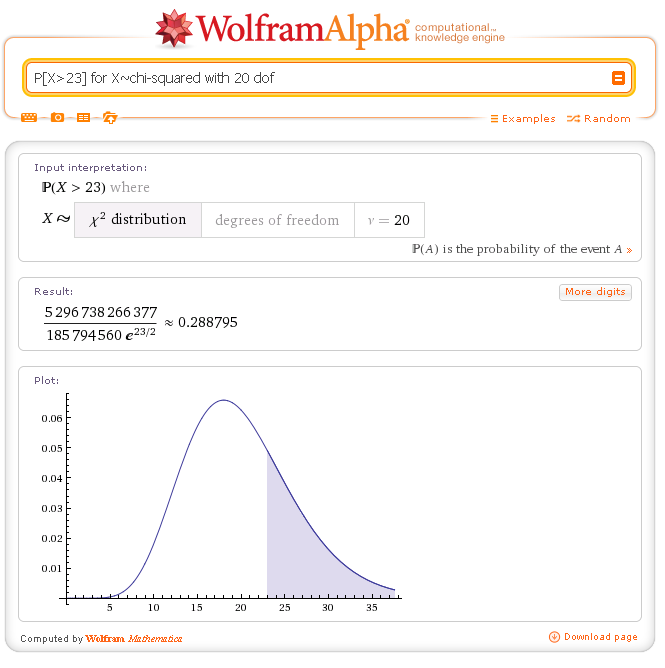
\includegraphics[width=9cm]{../fig/Tut07-03.png}
\end{center}
\caption{Wolfram Alpha para cálculos de probabilidad con $\chi^2$.}
\label{tut07:fig:ProbabilidadChiCuadradoWolframAlpha}
\end{figure}

\section{Ejercicios adicionales y soluciones.}
\label{tut07:sec:EjerciciosAdicionalesYSoluciones}

\subsection*{Ejercicios adicionales}
\label{tut07:subsec:EjerciciosAdicionales}

%\pendiente	

\begin{ejercicio}
\label{tut06:ejercicio16}

Cada uno de los siguientes ficheros contiene una muestra de una población normal. Usa los datos del fichero para contrastar la hipótesis nula que se indica, al correspondiente nivel de significación. Calcula siempre el p-valor del contraste.

\begin{enumerate}


%% Media con muestra grande.

  \item

  Fichero \fichero{../datos/Tut07-EjAdicionales-Contrastes01.csv}{Tut07-EjAdicionales-Contrastes01.csv}\\
  Hipótesis nula: $H_0=\{\mu\neq12.5\}$.
  Nivel de significación: $95\%$.


%% Media con muestra pequeña.

  \item

  Fichero \fichero{../datos/Tut07-EjAdicionales-Contrastes02.csv}{Tut07-EjAdicionales-Contrastes02.csv}\\
  Hipótesis nula: $H_0=\{\mu < -4.1\}$.
  Nivel de significación: $95\%$ y también $90\%$.


%% Varianza.

  \item

  Fichero \fichero{../datos/Tut07-EjAdicionales-Contrastes03.csv}{Tut07-EjAdicionales-Contrastes03.csv}\\
  Hipótesis nula: $H_0=\{\sigma^2 \neq 1.95\}$.
  Nivel de significación: $95\%$.



\end{enumerate}

\qed
\end{ejercicio}
%%##########################################



\subsection*{Soluciones de algunos ejercicios}
\label{tut07:subsec:SolucionesAlgunosEjercicios}


\paragraph{\bf $\bullet$ Ejercicio \ref{tut07:ejercicio01}, pág. \pageref{tut07:ejercicio01}}
\label{tut07:ejercicio01:sol}\quad\\

\begin{enumerate}
  \item A partir de los datos de la muestra calculamos el valor del estadístico:
\begin{knitrout}
\definecolor{shadecolor}{rgb}{0.969, 0.969, 0.969}\color{fgcolor}\begin{kframe}
\begin{alltt}
\hlstd{mu0} \hlkwb{=} \hlnum{2.5}
\hlstd{barX} \hlkwb{=} \hlnum{2.52}
\hlstd{n} \hlkwb{=} \hlnum{10000}
\hlstd{s} \hlkwb{=} \hlnum{0.5}
\hlstd{(estadistico} \hlkwb{=} \hlstd{(barX} \hlopt{-} \hlstd{mu0)} \hlopt{/} \hlstd{(s}\hlopt{/}\hlkwd{sqrt}\hlstd{(n)))}
\end{alltt}
\begin{verbatim}
## [1] 4
\end{verbatim}
\end{kframe}
\end{knitrout}
    Y ahora el p-valor es inmediato:
\begin{knitrout}
\definecolor{shadecolor}{rgb}{0.969, 0.969, 0.969}\color{fgcolor}\begin{kframe}
\begin{alltt}
\hlstd{(pValor} \hlkwb{=} \hlnum{1} \hlopt{-} \hlkwd{pnorm}\hlstd{(estadistico))}
\end{alltt}
\begin{verbatim}
## [1] 0.000031671
\end{verbatim}
\end{kframe}
\end{knitrout}

  \item  En la Ecuación \ref{curso-cap07:ecu:RegionRechazoMediaZColaDerecha} del libro (pág. \pageref{curso-cap07:ecu:RegionRechazoMediaZColaDerecha}) hemos visto que la región de rechazo se define así:
  \[R=\left\{\dfrac{\bar X-\mu_0}{\dfrac{s}{\sqrt{n}}} > z_{\alpha}\right\}\]
  Despejando de aquí $\bar X$ se obtiene:
  \[\bar X  > \mu_0 + z_{\alpha}\cdot \dfrac{s}{\sqrt{n}}\]
  Recordemos que en este ejemplo $\mu_0 = 2.5$, $n = 100$, $s = 0.5$, así que
\begin{knitrout}
\definecolor{shadecolor}{rgb}{0.969, 0.969, 0.969}\color{fgcolor}\begin{kframe}
\begin{alltt}
\hlstd{mu0} \hlkwb{=} \hlnum{2.5}
\hlstd{n} \hlkwb{=} \hlnum{100}
\hlstd{s} \hlkwb{=} \hlnum{0.5}
\hlstd{nc} \hlkwb{=} \hlnum{0.95}
\hlstd{alfa} \hlkwb{=} \hlnum{1} \hlopt{-} \hlstd{nc}
\hlstd{zAlfa} \hlkwb{=} \hlkwd{qnorm}\hlstd{(}\hlnum{1} \hlopt{-} \hlstd{alfa)}

\hlstd{mu0} \hlopt{+}  \hlstd{zAlfa} \hlopt{*} \hlstd{s} \hlopt{/}\hlkwd{sqrt}\hlstd{(n)}
\end{alltt}
\begin{verbatim}
## [1] 2.5822
\end{verbatim}
\end{kframe}
\end{knitrout}
  En consecuencia rechazaremos $H_0$ con cualquier valor de $\bar X$ mayor que 2.58224.


  \item La hipótesis nula es:
  \[H_0=\{\mu > 25\}\]
  y para realizar el contraste calculamos el estadistico a partir de los datos muestrales:
\begin{knitrout}
\definecolor{shadecolor}{rgb}{0.969, 0.969, 0.969}\color{fgcolor}\begin{kframe}
\begin{alltt}
\hlstd{mu0} \hlkwb{=} \hlnum{25}
\hlstd{n} \hlkwb{=} \hlnum{200}
\hlstd{barX} \hlkwb{=} \hlnum{26}
\hlstd{s} \hlkwb{=} \hlnum{7}
\hlstd{(Estadistico} \hlkwb{=} \hlstd{(barX} \hlopt{-} \hlstd{mu0)}\hlopt{/}\hlstd{(s} \hlopt{/} \hlkwd{sqrt}\hlstd{(n)))}
\end{alltt}
\begin{verbatim}
## [1] 2.0203
\end{verbatim}
\end{kframe}
\end{knitrout}
  Y a partir de aquí el p-valor:
\begin{knitrout}
\definecolor{shadecolor}{rgb}{0.969, 0.969, 0.969}\color{fgcolor}\begin{kframe}
\begin{alltt}
\hlstd{(pValor} \hlkwb{=} \hlnum{1} \hlopt{-} \hlkwd{pnorm}\hlstd{(Estadistico))}
\end{alltt}
\begin{verbatim}
## [1] 0.021676
\end{verbatim}
\end{kframe}
\end{knitrout}
  Puesto que el p-valor es menor que $0.05$ rechazamos la hipótesis nula al $95\%$. Pero como el p-valor es mayor que $0.01$, no rechazamos $H_0$ al $99\%$.


\end{enumerate}



\paragraph{\bf $\bullet$ Ejercicio \ref{tut07:ejercicio02}, pág. \pageref{tut07:ejercicio02}}
\label{tut07:ejercicio02:sol}\quad\\

\begin{enumerate}
  \item La flecha roja indica el resultado que obtenemos con Wolfram Alpha.
    \begin{center}
	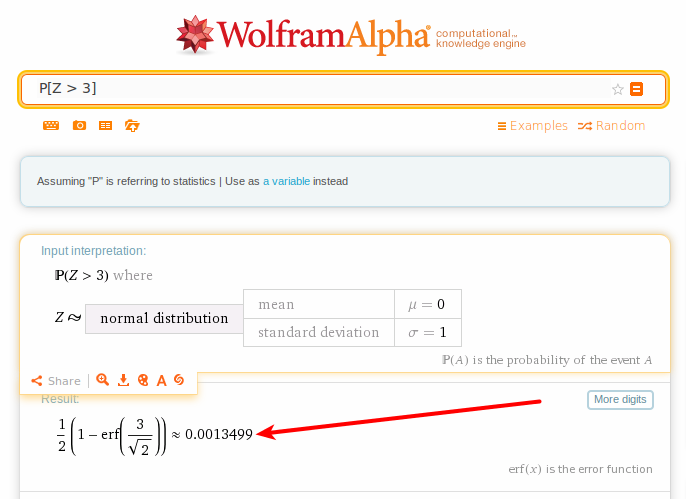
\includegraphics[width=14cm]{../fig/Tut07-08.png}
    \end{center}

  \item Y aquí está el resultado en la {\em Calculadora de Probabilidades} de GeoGebra.
    \begin{center}
	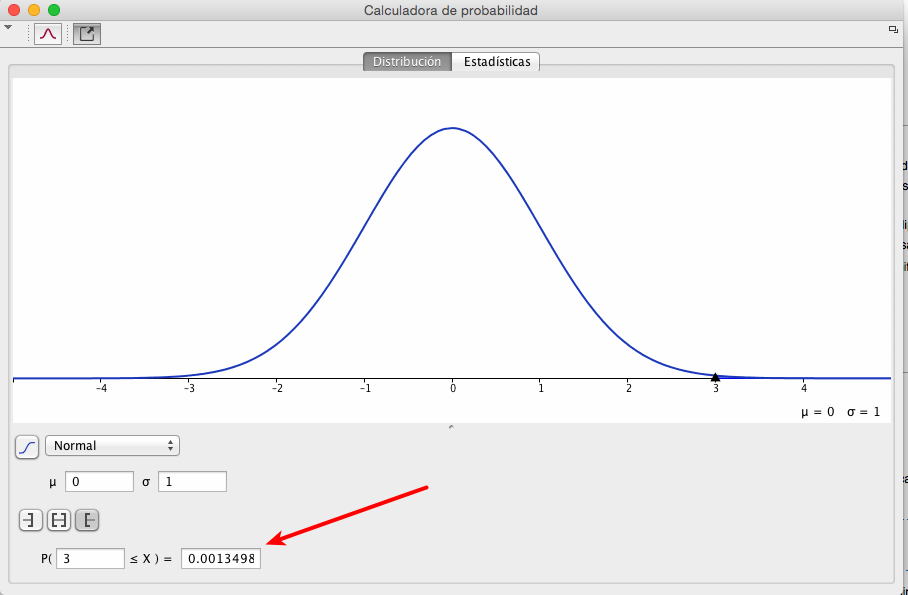
\includegraphics[width=14cm]{../fig/Tut07-09.png}
    \end{center}

   \item Lo más parecido a hacer ese ejercicio con R es ejecutar estos comandos, uno tras otro, en la {\em Línea de entrada} de GeoGebra:
   \begin{verbatim}
    mu0 = 25
    n = 200
    barX = 26
    s = 7
    estadistico = (barX - mu0)/(s / sqrt(n))
    1 - Normal[0, 1, estadistico]
   \end{verbatim}
   Todos deberían resultar evidentes, salvo quizá el último. La función {\tt Normal} es la versión GeoGebra de la función {\tt pnorm} de R. Si además tienes la precaución de seleccionar un número alto de cifras para el redondeo, obtendrás el p-valor deseado en la {\em Vista Algebraica}:
    \begin{center}
	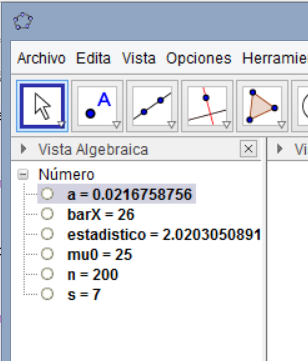
\includegraphics[width=5cm]{../fig/Tut07-12.png}
    \end{center}
   Otra posibilidad, dentro de GeoGebra, es usar la pestaña {\em Estadísticas} de la {\em Calculadora de Probabilidades}, como se muestra en esta figura:
    \begin{center}
	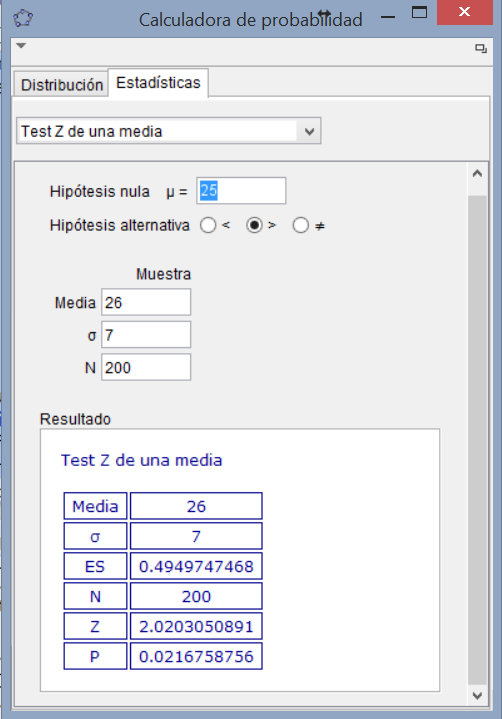
\includegraphics[width=7cm]{../fig/Tut07-13.png}
    \end{center}
   El resultado es, evidentemente, el mismo.

\end{enumerate}






\paragraph{\bf $\bullet$ Ejercicio \ref{tut07:ejercicio03}, pág. \pageref{tut07:ejercicio03}}
\label{tut07:ejercicio03:sol}\quad\\

El cálculo de la potencia es:
\begin{knitrout}
\definecolor{shadecolor}{rgb}{0.969, 0.969, 0.969}\color{fgcolor}\begin{kframe}
\begin{alltt}
\hlstd{n} \hlkwb{=} \hlnum{200}
\hlstd{delta} \hlkwb{=} \hlnum{0.2}
\hlstd{s} \hlkwb{=} \hlnum{7}
\hlstd{alfa} \hlkwb{=} \hlnum{0.05}
\hlstd{(zAlfa} \hlkwb{=} \hlkwd{qnorm}\hlstd{(}\hlnum{1}\hlopt{-} \hlstd{alfa))}
\end{alltt}
\begin{verbatim}
## [1] 1.6449
\end{verbatim}
\begin{alltt}
\hlstd{(potencia} \hlkwb{=} \hlnum{1} \hlopt{-} \hlkwd{pnorm}\hlstd{(zAlfa} \hlopt{-} \hlstd{delta} \hlopt{/} \hlstd{(s} \hlopt{/} \hlkwd{sqrt}\hlstd{(n)) ))}
\end{alltt}
\begin{verbatim}
## [1] 0.10734
\end{verbatim}
\end{kframe}
\end{knitrout}
La bajísima potencia que se obtiene se puede atribuir a la elevada dispersión con $s= 7$. Si rehaces los cálculos con $s=1$ verás que la potencia se eleva hasta casi el $90\%$.

El tamaño muestral, si se desea una potencia del 80\% se obtiene con estos cálculos:

\begin{knitrout}
\definecolor{shadecolor}{rgb}{0.969, 0.969, 0.969}\color{fgcolor}\begin{kframe}
\begin{alltt}
\hlstd{potenciaDeseada} \hlkwb{=} \hlnum{0.80}
\hlstd{delta} \hlkwb{=} \hlnum{0.2}
\hlstd{s} \hlkwb{=} \hlnum{7}
\hlstd{alfa} \hlkwb{=} \hlnum{0.05}

\hlstd{(zAlfa} \hlkwb{=} \hlkwd{qnorm}\hlstd{(}\hlnum{1}\hlopt{-} \hlstd{alfa))}
\end{alltt}
\begin{verbatim}
## [1] 1.6449
\end{verbatim}
\begin{alltt}
\hlstd{(zPot} \hlkwb{=} \hlkwd{qnorm}\hlstd{(}\hlnum{1} \hlopt{-} \hlstd{potenciaDeseada))}
\end{alltt}
\begin{verbatim}
## [1] -0.84162
\end{verbatim}
\begin{alltt}
\hlstd{(tamannoMuestra} \hlkwb{=}  \hlstd{( (s} \hlopt{/} \hlstd{delta)} \hlopt{*} \hlstd{(zAlfa} \hlopt{-} \hlstd{zPot))}\hlopt{^}\hlnum{2}\hlstd{)}
\end{alltt}
\begin{verbatim}
## [1] 7573.6
\end{verbatim}
\end{kframe}
\end{knitrout}
De nuevo, a causa de la elevada dispersión, necesitamos un tamaño muestral muy grande.



\paragraph{\bf $\bullet$ Ejercicio \ref{tut07:ejercicio04}, pág. \pageref{tut07:ejercicio04}}
\label{tut07:ejercicio04:sol}\quad\\
Introducimos el resto de los datos:
\begin{knitrout}
\definecolor{shadecolor}{rgb}{0.969, 0.969, 0.969}\color{fgcolor}\begin{kframe}
\begin{alltt}
\hlstd{mu0} \hlkwb{=} \hlnum{1000}
\hlstd{n} \hlkwb{=} \hlnum{100}
\hlstd{(s} \hlkwb{=} \hlkwd{sqrt}\hlstd{(}\hlnum{36.1}\hlstd{))}
\end{alltt}
\begin{verbatim}
## [1] 6.0083
\end{verbatim}
\end{kframe}
\end{knitrout}
y ahora vamos calculando el valor del estadístico para cada valor de $\bar X$:
\begin{knitrout}
\definecolor{shadecolor}{rgb}{0.969, 0.969, 0.969}\color{fgcolor}\begin{kframe}
\begin{alltt}
\hlstd{Xbar} \hlkwb{=} \hlnum{990}
\hlstd{(Estadistico} \hlkwb{=} \hlstd{(Xbar} \hlopt{-} \hlstd{mu0)} \hlopt{/} \hlstd{(s} \hlopt{/} \hlkwd{sqrt}\hlstd{(n)))}
\end{alltt}
\begin{verbatim}
## [1] -16.644
\end{verbatim}
\begin{alltt}
\hlstd{Xbar} \hlkwb{=} \hlnum{999.99}
\hlstd{(Estadistico} \hlkwb{=} \hlstd{(Xbar} \hlopt{-} \hlstd{mu0)} \hlopt{/} \hlstd{(s} \hlopt{/} \hlkwd{sqrt}\hlstd{(n)))}
\end{alltt}
\begin{verbatim}
## [1] -0.016644
\end{verbatim}
\begin{alltt}
\hlstd{Xbar} \hlkwb{=} \hlnum{1000.5}
\hlstd{(Estadistico} \hlkwb{=} \hlstd{(Xbar} \hlopt{-} \hlstd{mu0)} \hlopt{/} \hlstd{(s} \hlopt{/} \hlkwd{sqrt}\hlstd{(n)))}
\end{alltt}
\begin{verbatim}
## [1] 0.83218
\end{verbatim}
\end{kframe}
\end{knitrout}
La figura que pide el ejercicio podría ser algo como esto:
\begin{center}
    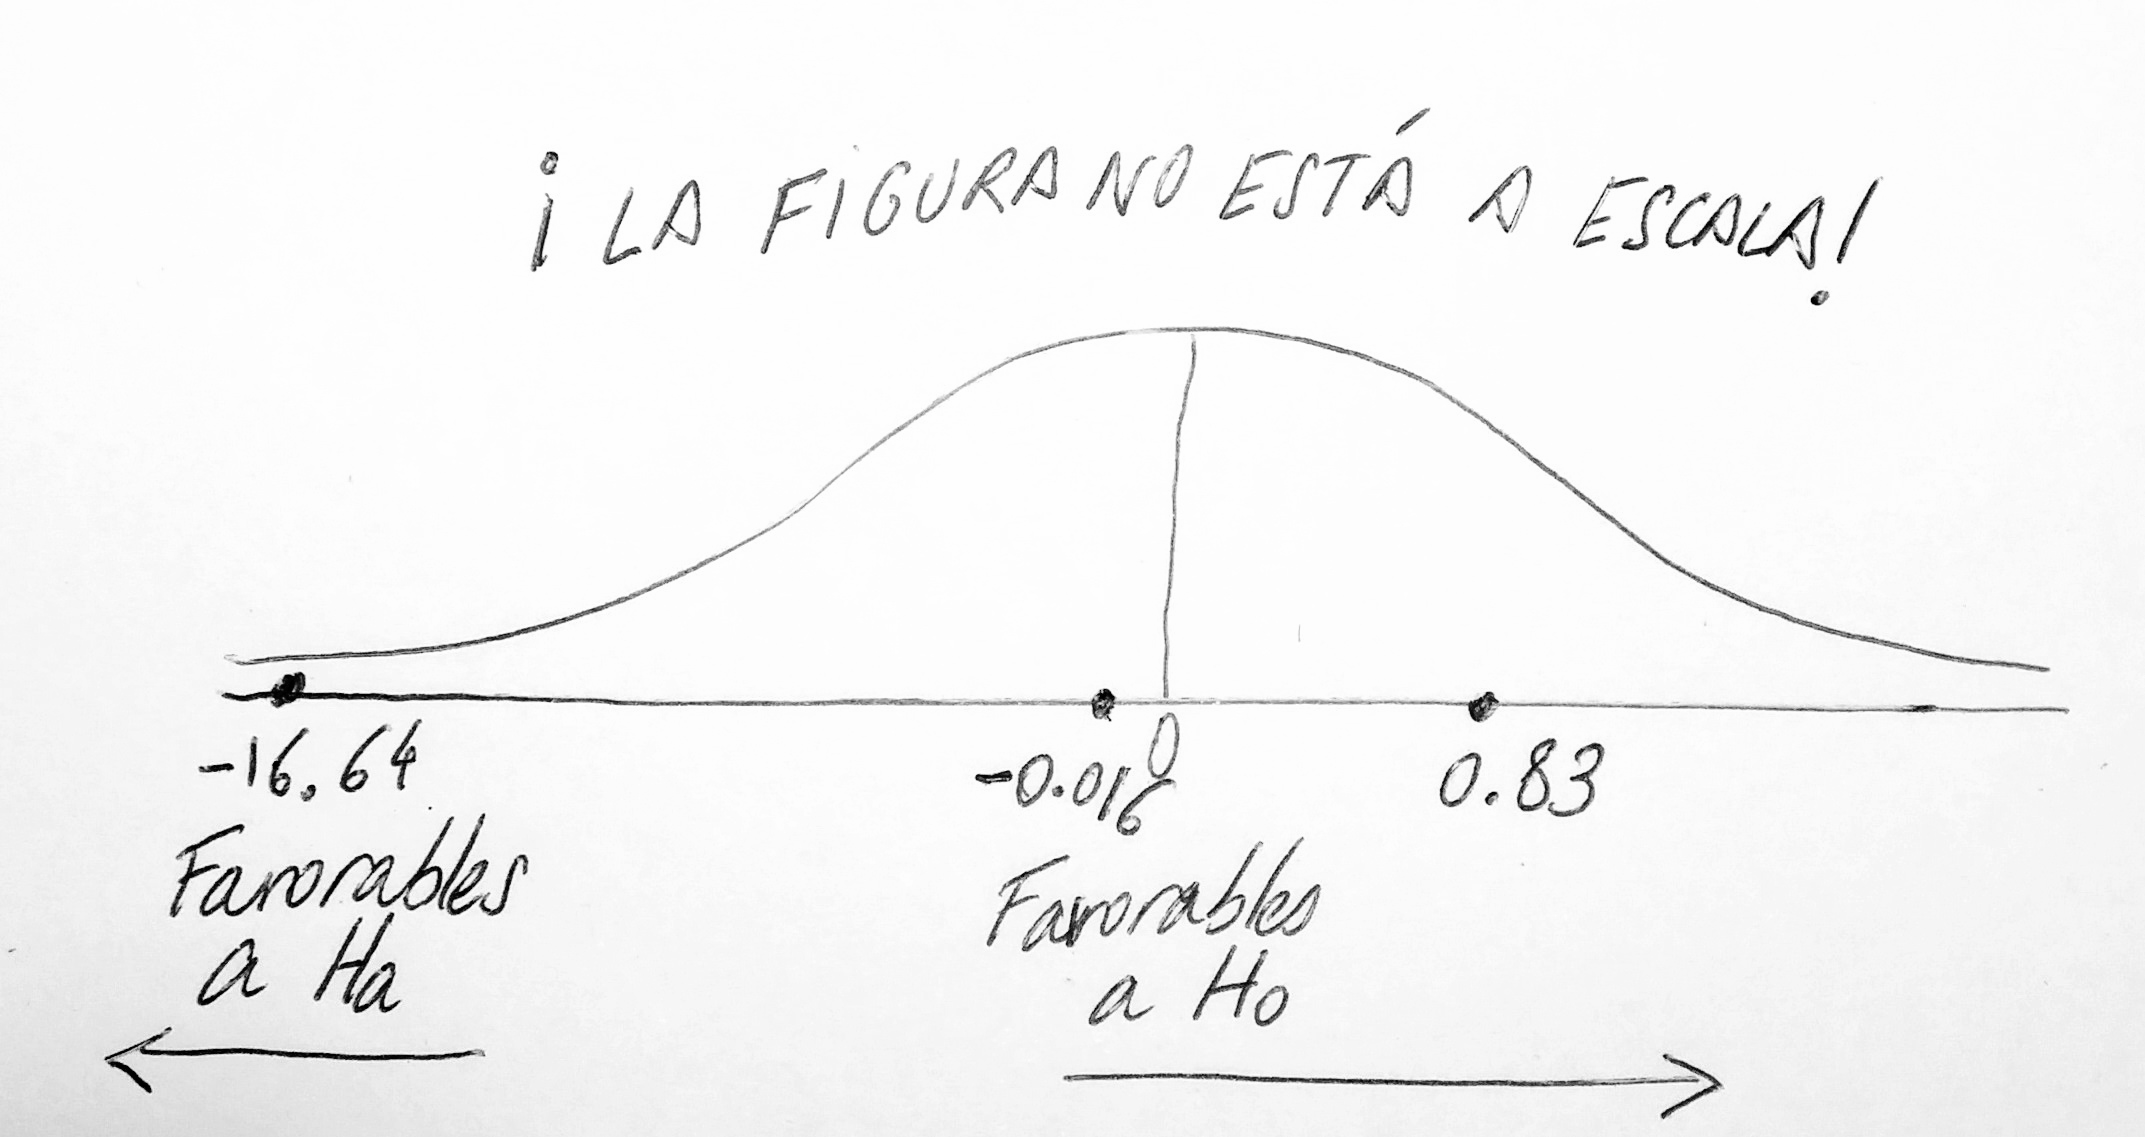
\includegraphics[width=14cm]{../fig/Tut07-14.png}
\end{center}
que indica, en términos muy generales, por dónde está la región de rechazo de $H_0$.

Vamos a calcular el p-valor para la media muestral original $\bar X= 998.5$:
\begin{knitrout}
\definecolor{shadecolor}{rgb}{0.969, 0.969, 0.969}\color{fgcolor}\begin{kframe}
\begin{alltt}
\hlstd{Xbar} \hlkwb{=} \hlnum{998.5}
\hlstd{(Estadistico} \hlkwb{=} \hlstd{(Xbar} \hlopt{-} \hlstd{mu0)} \hlopt{/} \hlstd{(s} \hlopt{/} \hlkwd{sqrt}\hlstd{(n)))}
\end{alltt}
\begin{verbatim}
## [1] -2.4965
\end{verbatim}
\end{kframe}
\end{knitrout}
En este caso, los valores favorables a $H_a$ son los de la cola {\bf izquierda} del estadístico. Por eso el p-valor es:
\begin{knitrout}
\definecolor{shadecolor}{rgb}{0.969, 0.969, 0.969}\color{fgcolor}\begin{kframe}
\begin{alltt}
  \hlstd{(pValor} \hlkwb{=} \hlkwd{pnorm}\hlstd{(Estadistico))}
\end{alltt}
\begin{verbatim}
## [1] 0.0062707
\end{verbatim}
\end{kframe}
\end{knitrout}

\paragraph{\bf $\bullet$ Ejercicio \ref{tut07:ejercicio05}, pág. \pageref{tut07:ejercicio05}}
\label{tut07:ejercicio05:sol}\quad\\

Deshaciendo la tipificación es:
\begin{knitrout}
\definecolor{shadecolor}{rgb}{0.969, 0.969, 0.969}\color{fgcolor}\begin{kframe}
\begin{alltt}
\hlstd{mu0} \hlkwb{=} \hlnum{1000}
\hlstd{n} \hlkwb{=} \hlnum{100}
\hlstd{(s} \hlkwb{=} \hlkwd{sqrt}\hlstd{(}\hlnum{36.1}\hlstd{))}
\end{alltt}
\begin{verbatim}
## [1] 6.0083
\end{verbatim}
\begin{alltt}
\hlstd{nc} \hlkwb{=} \hlnum{0.99}
\hlstd{(alfa} \hlkwb{=} \hlnum{1} \hlopt{-} \hlstd{nc)}
\end{alltt}
\begin{verbatim}
## [1] 0.01
\end{verbatim}
\begin{alltt}
\hlstd{(zUnoMenosAlfa} \hlkwb{=} \hlkwd{qnorm}\hlstd{(alfa))}
\end{alltt}
\begin{verbatim}
## [1] -2.3263
\end{verbatim}
\begin{alltt}
\hlstd{(destipificado} \hlkwb{=} \hlstd{mu0} \hlopt{+} \hlstd{zUnoMenosAlfa} \hlopt{*} \hlstd{s} \hlopt{/} \hlkwd{sqrt}\hlstd{(n))}
\end{alltt}
\begin{verbatim}
## [1] 998.6
\end{verbatim}
\end{kframe}
\end{knitrout}
Si el peso medio muestral es menor que esta cantidad, el inspector rechazará $H_0$ y concluirá que el fabricante está incluyendo menos peso del que anuncia.

\paragraph{\bf $\bullet$ Ejercicio \ref{tut07:ejercicio06}, pág. \pageref{tut07:ejercicio06}}
\label{tut07:ejercicio06:sol}\quad\\

El valor del estadístico para $\bar X=1000.3$ se obtiene con:
\begin{knitrout}
\definecolor{shadecolor}{rgb}{0.969, 0.969, 0.969}\color{fgcolor}\begin{kframe}
\begin{alltt}
\hlstd{mu0} \hlkwb{=} \hlnum{1000}
\hlstd{n} \hlkwb{=} \hlnum{100}
\hlstd{(s} \hlkwb{=} \hlkwd{sqrt}\hlstd{(}\hlnum{36.1}\hlstd{))}
\end{alltt}
\begin{verbatim}
## [1] 6.0083
\end{verbatim}
\begin{alltt}
\hlstd{Xbar} \hlkwb{=} \hlnum{1000.3}
\hlstd{(Estadistico} \hlkwb{=} \hlkwd{abs}\hlstd{(Xbar} \hlopt{-} \hlstd{mu0)} \hlopt{/} \hlstd{(s} \hlopt{/} \hlkwd{sqrt}\hlstd{(n)))}
\end{alltt}
\begin{verbatim}
## [1] 0.49931
\end{verbatim}
\end{kframe}
\end{knitrout}

Para que el estadístico valga $2$, puesto que interviene el valor absoluto, puede ser
\[
\dfrac{\bar X - \mu_0}{s \sqrt{n}} = 2,
\]
pero, claro, también:
\[
\dfrac{\bar X - \mu_0}{s \sqrt{n}} = -2.
\]
Sustituyendo los valores muestrales se obtienen los dos posibles valores de $\bar X$:

\begin{knitrout}
\definecolor{shadecolor}{rgb}{0.969, 0.969, 0.969}\color{fgcolor}\begin{kframe}
\begin{alltt}
\hlstd{mu0} \hlopt{+} \hlkwd{c}\hlstd{(}\hlopt{-}\hlnum{2}\hlstd{,} \hlnum{2}\hlstd{)} \hlopt{*} \hlstd{(s}\hlopt{/}\hlkwd{sqrt}\hlstd{(n))}
\end{alltt}
\begin{verbatim}
## [1]  998.8 1001.2
\end{verbatim}
\end{kframe}
\end{knitrout}

La cola derecha, los valores positivos del estadístico, corresponde a medias muestrales superiores a lo que anuncia el fabricante. Es decir a exceso de producto envasado. La cola izquierda, la de los valores negativos del estadístico, corresponde a medias muestrales menores de lo anunciado y representa el riesgo de sufrir la sanción del inspector.


\paragraph{\bf $\bullet$ Ejercicio \ref{tut07:ejercicio07}, pág. \pageref{tut07:ejercicio07}}
\label{tut07:ejercicio07:sol}\quad\\

\begin{enumerate}
  \item La razón para usar {\tt 1 - pnorm} es que queremos calcular la probabilidad de la cola derecha. Y luego la multiplicamos por $2$ para obtener la suma de las probabilidades de ambas colas. De hecho, si te equivocas aquí, y usas {\tt pnorm}, obtendrás un p-valor mayor que $1$, que no tiene sentido (recuerda que un p-valor es siempre una probabilidad).

  \item El estadístico que usa el inspector es:
\begin{knitrout}
\definecolor{shadecolor}{rgb}{0.969, 0.969, 0.969}\color{fgcolor}\begin{kframe}
\begin{alltt}
  \hlstd{mu0} \hlkwb{=} \hlnum{1000}
  \hlstd{n} \hlkwb{=} \hlnum{100}
  \hlstd{Xbar} \hlkwb{=} \hlnum{999.7}
  \hlstd{(s} \hlkwb{=} \hlkwd{sqrt}\hlstd{(}\hlnum{20.2}\hlstd{))}
\end{alltt}
\begin{verbatim}
## [1] 4.4944
\end{verbatim}
\begin{alltt}
  \hlstd{(Estadistico} \hlkwb{=} \hlstd{(Xbar} \hlopt{-} \hlstd{mu0)} \hlopt{/} \hlstd{(s} \hlopt{/} \hlkwd{sqrt}\hlstd{(n)))}
\end{alltt}
\begin{verbatim}
## [1] -0.66749
\end{verbatim}
\end{kframe}
\end{knitrout}
  y el p-valor se calcula con:
\begin{knitrout}
\definecolor{shadecolor}{rgb}{0.969, 0.969, 0.969}\color{fgcolor}\begin{kframe}
\begin{alltt}
\hlkwd{pnorm}\hlstd{(Estadistico)}
\end{alltt}
\begin{verbatim}
## [1] 0.25223
\end{verbatim}
\end{kframe}
\end{knitrout}
  Aunque el peso muestral es menor de $1000$ gramos, el p-valor es muy alto, así que el inspector no rechaza $H_0$ y por tanto, ahora, no tiene razones basadas en los datos para sospechar que el fabricante esté envasando menos producto del anunciado.

  \item Si hacemos $\bar X=999.1$ entonces el inspector calcula el p-valor así:
\begin{knitrout}
\definecolor{shadecolor}{rgb}{0.969, 0.969, 0.969}\color{fgcolor}\begin{kframe}
\begin{alltt}
\hlstd{Xbar} \hlkwb{=} \hlnum{999.1}
\hlstd{(Estadistico} \hlkwb{=} \hlstd{(Xbar} \hlopt{-} \hlstd{mu0)} \hlopt{/} \hlstd{(s} \hlopt{/} \hlkwd{sqrt}\hlstd{(n)))}
\end{alltt}
\begin{verbatim}
## [1] -2.0025
\end{verbatim}
\begin{alltt}
\hlstd{(pValorInspector} \hlkwb{=} \hlkwd{pnorm}\hlstd{(Estadistico))}
\end{alltt}
\begin{verbatim}
## [1] 0.022617
\end{verbatim}
\end{kframe}
\end{knitrout}
    El fabricante, por su parte, calcula el p-valor así:
\begin{knitrout}
\definecolor{shadecolor}{rgb}{0.969, 0.969, 0.969}\color{fgcolor}\begin{kframe}
\begin{alltt}
\hlstd{Xbar} \hlkwb{=} \hlnum{999.1}
\hlstd{(Estadistico} \hlkwb{=} \hlkwd{abs}\hlstd{(Xbar} \hlopt{-} \hlstd{mu0)} \hlopt{/} \hlstd{(s} \hlopt{/} \hlkwd{sqrt}\hlstd{(n)))}
\end{alltt}
\begin{verbatim}
## [1] 2.0025
\end{verbatim}
\begin{alltt}
\hlstd{(pValorFabricante} \hlkwb{=} \hlnum{2} \hlopt{*} \hlstd{(}\hlnum{1} \hlopt{-} \hlkwd{pnorm}\hlstd{(Estadistico)))}
\end{alltt}
\begin{verbatim}
## [1] 0.045234
\end{verbatim}
\end{kframe}
\end{knitrout}
    Si estuviéramos usando un nivel de significación del 95\%, ambos rechazarían la hipótesis nula, pero por un margen distinto.

  \item Los cálculos anteriores indican que, en efecto, eso puede suceder. Dejamos  para el lector la tarea de experimentar con el código para buscarlos.
\end{enumerate}



\paragraph{\bf $\bullet$ Ejercicio \ref{tut07:ejercicio08}, pág. \pageref{tut07:ejercicio08}}
\label{tut07:ejercicio08:sol}\quad\\

El código para el cálculo del p-valor es:
\begin{knitrout}
\definecolor{shadecolor}{rgb}{0.969, 0.969, 0.969}\color{fgcolor}\begin{kframe}
\begin{alltt}
\hlstd{datos} \hlkwb{=} \hlkwd{read.table}\hlstd{(}\hlkwc{file} \hlstd{=} \hlstr{"../datos/Tut07-Ejercicio-ContrasteMedia.csv"}\hlstd{)[ ,}\hlnum{1}\hlstd{]}
\hlstd{(n} \hlkwb{=} \hlkwd{length}\hlstd{(datos))}
\end{alltt}
\begin{verbatim}
## [1] 300
\end{verbatim}
\begin{alltt}
\hlstd{(Xbar} \hlkwb{=} \hlkwd{mean}\hlstd{(datos))}
\end{alltt}
\begin{verbatim}
## [1] 27.1
\end{verbatim}
\begin{alltt}
\hlstd{(s} \hlkwb{=} \hlkwd{sd}\hlstd{(datos))}
\end{alltt}
\begin{verbatim}
## [1] 0.8
\end{verbatim}
\begin{alltt}
\hlstd{mu0} \hlkwb{=} \hlnum{27}
\hlstd{(Estadistico} \hlkwb{=} \hlstd{(Xbar} \hlopt{-} \hlstd{mu0)} \hlopt{/} \hlstd{(s} \hlopt{/} \hlkwd{sqrt}\hlstd{(n)))}
\end{alltt}
\begin{verbatim}
## [1] 2.1651
\end{verbatim}
\begin{alltt}
\hlstd{(pValor} \hlkwb{=} \hlnum{1} \hlopt{-} \hlkwd{pnorm}\hlstd{(Estadistico))}
\end{alltt}
\begin{verbatim}
## [1] 0.015191
\end{verbatim}
\end{kframe}
\end{knitrout}
Y la conclusión, como ves, depende del nivel de significación que se utilice.

\paragraph{\bf $\bullet$ Ejercicio \ref{tut07:ejercicio09}, pág. \pageref{tut07:ejercicio09}}
\label{tut07:ejercicio09:sol}\quad\\

\begin{enumerate}

  \item Las hipótesis nula y alternativa son, respectivamente:
  \[H_0=\{\mu \geq 0.29 \}\mbox{ y }H_a=\{\mu < 0.29 \}.\]
  Para realizar el contraste empezamos por crear un vector con los datos muestrales, a partir del cual hacemos los cálculos necesarios para obtener el estadístico:
\begin{knitrout}
\definecolor{shadecolor}{rgb}{0.969, 0.969, 0.969}\color{fgcolor}\begin{kframe}
\begin{alltt}
\hlstd{muestra} \hlkwb{=} \hlkwd{c}\hlstd{(}\hlnum{0.316}\hlstd{,} \hlnum{0.295}\hlstd{,} \hlnum{0.304}\hlstd{,} \hlnum{0.263}\hlstd{,} \hlnum{0.25}\hlstd{)}
\hlstd{(n} \hlkwb{=} \hlkwd{length}\hlstd{(muestra))}
\end{alltt}
\begin{verbatim}
## [1] 5
\end{verbatim}
\begin{alltt}
\hlstd{(barX} \hlkwb{=} \hlkwd{mean}\hlstd{(muestra))}
\end{alltt}
\begin{verbatim}
## [1] 0.2856
\end{verbatim}
\begin{alltt}
\hlstd{(s} \hlkwb{=} \hlkwd{sd}\hlstd{(muestra))}
\end{alltt}
\begin{verbatim}
## [1] 0.02797
\end{verbatim}
\begin{alltt}
\hlstd{mu0} \hlkwb{=} \hlnum{0.29}
\hlstd{(Estadistico} \hlkwb{=} \hlstd{(barX} \hlopt{-} \hlstd{mu0)} \hlopt{/} \hlstd{(s}\hlopt{/}\hlkwd{sqrt}\hlstd{(n)))}
\end{alltt}
\begin{verbatim}
## [1] -0.35176
\end{verbatim}
\begin{alltt}
\hlstd{ns} \hlkwb{=} \hlnum{0.95}
\hlstd{alfa} \hlkwb{=} \hlnum{1} \hlopt{-} \hlstd{ns}
\end{alltt}
\end{kframe}
\end{knitrout}
  El p-valor es la probabilidad de la cola izquierda de este estadístico en la distribución $t$ de Student correspondiente:
\begin{knitrout}
\definecolor{shadecolor}{rgb}{0.969, 0.969, 0.969}\color{fgcolor}\begin{kframe}
\begin{alltt}
\hlstd{(pValor} \hlkwb{=} \hlkwd{pt}\hlstd{(Estadistico,} \hlkwc{df} \hlstd{= n} \hlopt{-} \hlnum{1}\hlstd{))}
\end{alltt}
\begin{verbatim}
## [1] 0.37138
\end{verbatim}
\end{kframe}
\end{knitrout}
  Y está claro que con ese p-valor no podemos rechazar la hipótesis nula. Es decir, que el investigador no tiene base experimental suficiente para concluir que el  tiempo de reacción medio del sujeto está por debajo de los $0.29$ segundos. La región de rechazo al $95\%$ la forman los valores del estadístico menores que:
\begin{knitrout}
\definecolor{shadecolor}{rgb}{0.969, 0.969, 0.969}\color{fgcolor}\begin{kframe}
\begin{alltt}
\hlstd{(tUnoMenosAlfa} \hlkwb{=} \hlkwd{qt}\hlstd{(alfa,} \hlkwc{df} \hlstd{= n}\hlopt{-}\hlnum{1}\hlstd{))}
\end{alltt}
\begin{verbatim}
## [1] -2.1318
\end{verbatim}
\end{kframe}
\end{knitrout}
  y de nuevo puedes ver que el estadístico que se ha obtenido no está en esa región de rechazo.

  \item Que la dosis sea la deseada significa que no sea ni mucho ni poco. Eso nos lleva a plantear una hipótesis nula bilateral:
      \[H_0=\{\mu = 500\}.\]
      Introducimos los valores de la muestra y hacemos el cálculo del estadístico (¡bilateral, recuerda!)
\begin{knitrout}
\definecolor{shadecolor}{rgb}{0.969, 0.969, 0.969}\color{fgcolor}\begin{kframe}
\begin{alltt}
  \hlstd{muestra} \hlkwb{=} \hlkwd{c}\hlstd{(}\hlnum{491}\hlstd{,} \hlnum{503}\hlstd{,} \hlnum{492}\hlstd{,} \hlnum{502}\hlstd{,} \hlnum{490}\hlstd{,} \hlnum{500}\hlstd{,} \hlnum{500}\hlstd{,} \hlnum{501}\hlstd{,}
        \hlnum{501}\hlstd{,} \hlnum{501}\hlstd{,} \hlnum{505}\hlstd{,} \hlnum{491}\hlstd{,} \hlnum{501}\hlstd{,} \hlnum{493}\hlstd{,} \hlnum{492}\hlstd{)}
  \hlstd{(n} \hlkwb{=} \hlkwd{length}\hlstd{(muestra))}
\end{alltt}
\begin{verbatim}
## [1] 15
\end{verbatim}
\begin{alltt}
  \hlstd{(barX} \hlkwb{=} \hlkwd{mean}\hlstd{(muestra))}
\end{alltt}
\begin{verbatim}
## [1] 497.53
\end{verbatim}
\begin{alltt}
  \hlstd{(s} \hlkwb{=} \hlkwd{sd}\hlstd{(muestra))}
\end{alltt}
\begin{verbatim}
## [1] 5.2762
\end{verbatim}
\begin{alltt}
  \hlstd{mu0} \hlkwb{=} \hlnum{500}
  \hlstd{(Estadistico} \hlkwb{=} \hlstd{(barX} \hlopt{-} \hlstd{mu0)} \hlopt{/} \hlstd{(s}\hlopt{/}\hlkwd{sqrt}\hlstd{(n)))}
\end{alltt}
\begin{verbatim}
## [1] -1.8107
\end{verbatim}
\begin{alltt}
  \hlstd{ns} \hlkwb{=} \hlnum{0.95}
  \hlstd{alfa} \hlkwb{=} \hlnum{1} \hlopt{-} \hlstd{ns}
  \hlstd{alfaMedios} \hlkwb{=} \hlstd{alfa} \hlopt{/} \hlnum{2}
\end{alltt}
\end{kframe}
\end{knitrout}

        Y el p-valor es:
\begin{knitrout}
\definecolor{shadecolor}{rgb}{0.969, 0.969, 0.969}\color{fgcolor}\begin{kframe}
\begin{alltt}
\hlstd{(pValor} \hlkwb{=} \hlnum{2} \hlopt{*} \hlstd{(}\hlnum{1} \hlopt{-} \hlkwd{pt}\hlstd{(}\hlkwd{abs}\hlstd{(Estadistico),} \hlkwc{df} \hlstd{= n} \hlopt{-} \hlnum{1}\hlstd{)))}
\end{alltt}
\begin{verbatim}
## [1] 0.091702
\end{verbatim}
\end{kframe}
\end{knitrout}
        El p-valor es, aunque por poco, mayor que $0.05$, así que no rechazamos $H_0$. La región de rechazo la forman aquellos valores del estadístico que están más lejos del origen que $t_{k; \alpha/2}$, es decir más lejos que:
\begin{knitrout}
\definecolor{shadecolor}{rgb}{0.969, 0.969, 0.969}\color{fgcolor}\begin{kframe}
\begin{alltt}
    \hlkwd{qt}\hlstd{(}\hlnum{1} \hlopt{-} \hlstd{alfaMedios,} \hlkwc{df}\hlstd{= n} \hlopt{-} \hlnum{1} \hlstd{)}
\end{alltt}
\begin{verbatim}
## [1] 2.1448
\end{verbatim}
\end{kframe}
\end{knitrout}


\end{enumerate}


\paragraph{\bf $\bullet$ Ejercicio \ref{tut07:ejercicio10}, pág. \pageref{tut07:ejercicio10}}
\label{tut07:ejercicio10:sol}\quad\\


\begin{knitrout}
\definecolor{shadecolor}{rgb}{0.969, 0.969, 0.969}\color{fgcolor}\begin{kframe}
\begin{alltt}
\hlstd{datos} \hlkwb{=} \hlkwd{read.table}\hlstd{(}\hlkwc{file} \hlstd{=} \hlstr{"../datos/Tut07-Ejercicio-ContrasteVarianza.csv"}\hlstd{)[,}\hlnum{1}\hlstd{]}
\hlstd{(n} \hlkwb{=} \hlkwd{length}\hlstd{(datos))}
\end{alltt}
\begin{verbatim}
## [1] 125
\end{verbatim}
\begin{alltt}
\hlstd{(Xbar} \hlkwb{=} \hlkwd{mean}\hlstd{(datos))} \hlcom{# Este dato no se usa en el contraste!!}
\end{alltt}
\begin{verbatim}
## [1] 12
\end{verbatim}
\begin{alltt}
\hlstd{(s} \hlkwb{=} \hlkwd{sd}\hlstd{(datos))}
\end{alltt}
\begin{verbatim}
## [1] 4.1049
\end{verbatim}
\begin{alltt}
\hlstd{sigma0} \hlkwb{=} \hlnum{3.7}
\hlstd{(Y} \hlkwb{=} \hlstd{(n}\hlopt{-}\hlnum{1}\hlstd{)} \hlopt{*} \hlstd{s}\hlopt{^}\hlnum{2} \hlopt{/} \hlstd{sigma0}\hlopt{^}\hlnum{2}\hlstd{)}
\end{alltt}
\begin{verbatim}
## [1] 152.62
\end{verbatim}
\begin{alltt}
\hlstd{k} \hlkwb{=} \hlstd{n} \hlopt{-} \hlnum{1}
\hlstd{(pvalor} \hlkwb{=} \hlnum{2}\hlopt{*}\hlstd{(}\hlnum{1} \hlopt{-} \hlkwd{pchisq}\hlstd{(Y,} \hlkwc{df} \hlstd{= k)))}
\end{alltt}
\begin{verbatim}
## [1] 0.082648
\end{verbatim}
\end{kframe}
\end{knitrout}

%\paragraph{\bf $\bullet$ Ejercicio \ref{tut07:ejercicio11}, pág. \pageref{tut07:ejercicio11}}
%\label{tut07:ejercicio11:sol}\quad\\
%
%<<t07ej11sol>>=
%n = 10000
%@


\paragraph{\bf $\bullet$ Ejercicio \ref{tut07:ejercicio12}, pág. \pageref{tut07:ejercicio12}}
\label{tut07:ejercicio12:sol}\quad\\

Comprueba si obtienes estos valores:
\[n=10, \quad, \bar X\approx 9.01,\quad s\approx 1.631938.\]
El estadístico del contraste vale
\[\dfrac{\bar X-\mu_0}{\dfrac{s}{\sqrt{n}}}\approx 1.957121.\]
Y el p-valor es:
\[pValor\approx 0.04101152\]

%<<t07ej12sol>>=
%n = 10000
%@


%\paragraph{\bf $\bullet$ Ejercicio \ref{tut07:ejercicio13}, pág. \pageref{tut07:ejercicio13}}
%\label{tut07:ejercicio13:sol}\quad\\
%
%<<t07ej13sol>>=
%n = 10000
%@
%





%#########################################################################################
%#########################################################################################
\vspace{2cm} \hrule
\quad\\
Fin del Tutorial07. ¡Gracias por la atención!

%\newpage
%\addcontentsline{toc}{section}{Guía de trabajo.}
%\includepdf[pages={1-},scale=0.90]{07-GuiaDeTrabajo.pdf}



\end{document} 
